% /*
%  * ----------------------------------------------------------------------------
%  * "THE BEER-WARE LICENSE" (Revision 42):
%  * <michi.wieland@hotmail.com> wrote this file. As long as you retain this notice you
%%  * can do whatever you want with this stuff. If we meet some day, and you think
%  * this stuff is worth it, you can buy me a beer in return. Michael Wieland
%  * ----------------------------------------------------------------------------
%  */

\documentclass[
a4paper,
oneside,
10pt,
fleqn,
headsepline,
toc=listofnumbered, 
bibliography=totocnumbered]{scrartcl}

% deutsche Trennmuster etc.
\usepackage[T1]{fontenc}
\usepackage[utf8]{inputenc}
\usepackage[english, ngerman]{babel} % \selectlanguage{english} if  needed
\usepackage{lmodern} % use modern latin fonts

% Custom commands
\newcommand{\AUTHOR}{Michael Wieland}
\newcommand{\INSTITUTE}{Hochschule für Technik Rapperswil}
\newcommand{\GITHUB}{https://github.com/michiwieland/hsr-zusammenfassungen}
\newcommand{\LICENSEURL}{https://en.wikipedia.org/wiki/Beerware}
\newcommand{\LICENSE}{
"THE BEER-WARE LICENSE" (Revision 42):
<michi.wieland@hotmail.com> wrote this file. As long as you retain this notice you
can do whatever you want with this stuff. If we meet some day, and you think
this stuff is worth it, you can buy me a beer in return. Michael Wieland	
}

% Jede Überschrift 1 auf neuer Seite
\let\stdsection\section
\renewcommand\section{\clearpage\stdsection}

% Multiple Authors
\usepackage{authblk}

% Include external pdf
\usepackage{pdfpages}

% Layout / Seitenränder
\usepackage{geometry}

% Inhaltsverzeichnis
\usepackage{makeidx} 
\makeindex

\usepackage{url}
\usepackage[pdfborder={0 0 0}]{hyperref}
\usepackage[all]{hypcap}
\usepackage{hyperxmp} % for license metadata

% Glossar und Abkürzungsverzeichnis
\usepackage[acronym,toc,nopostdot]{glossaries}
\glossarystyle{altlist}
\usepackage{xparse}
\DeclareDocumentCommand{\newdualentry}{ O{} O{} m m m m } {
	\newglossaryentry{gls-#3}{
		name={#4 : #5},
		text={#5\glsadd{#3}},
		description={#6},
		#1
	}
	\makeglossaries
	\newacronym[see={[Siehe:]{gls-#3}},#2]{#3}{#4}{#5\glsadd{gls-#3}}
}
\makeglossaries

% Mathematik
\usepackage{amsmath}
\usepackage{amssymb}
\usepackage{amsfonts}
\usepackage{enumitem}

% Images
\usepackage{graphicx}
\graphicspath{{images/}} % default paths

% Boxes
\usepackage{fancybox}

%Tables
\usepackage{tabu}
\usepackage{booktabs} % toprule, midrule, bottomrule
\usepackage{array} % for matrix tables

% Multi Columns
\usepackage{multicol}

% Header and footer
\usepackage{scrlayer-scrpage}
\setkomafont{pagehead}{\normalfont}
\setkomafont{pagefoot}{\normalfont}
\automark*{section}
\clearpairofpagestyles
\ihead{\headmark}
\ohead{\AUTHOR}
\cfoot{\pagemark}

% Pseudocode
\usepackage{algorithmic}
\usepackage[linesnumbered,ruled]{algorithm2e}

% Code Listings
\usepackage{listings}
\usepackage{color}
\usepackage{beramono}

\definecolor{bluekeywords}{rgb}{0,0,1}
\definecolor{greencomments}{rgb}{0,0.5,0}
\definecolor{redstrings}{rgb}{0.64,0.08,0.08}
\definecolor{xmlcomments}{rgb}{0.5,0.5,0.5}
\definecolor{types}{rgb}{0.17,0.57,0.68}

\lstdefinestyle{visual-studio-style}{
	language=[Sharp]C,
	columns=flexible,
	showstringspaces=false,
	basicstyle=\footnotesize\ttfamily, 
	commentstyle=\color{greencomments},
	morekeywords={partial, var, value, get, set},
	keywordstyle=\bfseries\color{bluekeywords},
	stringstyle=\color{redstrings},
	breaklines=true,
	breakatwhitespace=true,
	tabsize=4,
	numbers=left,
	numberstyle=\tiny\color{black},
	frame=lines,
	showspaces=false,
	showtabs=false,
	escapeinside={£}{£},
}

\definecolor{DarkPurple}{rgb}{0.4, 0.1, 0.4}
\definecolor{DarkCyan}{rgb}{0.0, 0.5, 0.4}
\definecolor{LightLime}{rgb}{0.3, 0.5, 0.4}
\definecolor{Blue}{rgb}{0.0, 0.0, 1.0}

\lstdefinestyle{cevelop-style}{
	language=C++,  
	columns=flexible,
	showstringspaces=false,     
	basicstyle=\footnotesize\ttfamily, 
	keywordstyle=\bfseries\color{DarkPurple},
	commentstyle=\color{LightLime},
	stringstyle=\color{Blue}, 
	escapeinside={£}{£}, % latex scope within code      
	breaklines=true,
	breakatwhitespace=true,
	showspaces=false,
	showtabs=false,
	tabsize=4,
	morekeywords={include,ifndef,define},
	numbers=left,
	numberstyle=\tiny\color{black},
	frame=lines,
}

\lstdefinestyle{eclipse-style}{
	language=Java,  
	columns=flexible,
	showstringspaces=false,     
	basicstyle=\footnotesize\ttfamily, 
	keywordstyle=\bfseries\color{DarkPurple},
	commentstyle=\color{LightLime},
	stringstyle=\color{Blue}, 
	escapeinside={£}{£}, % latex scope within code      
	breaklines=true,
	breakatwhitespace=true,
	showspaces=false,
	showtabs=false,
	tabsize=4,
	morekeywords={length},
	numbers=left,
	numberstyle=\tiny\color{black},
	frame=lines,
}
\lstset{style=eclipse-style}



% Theorems \begin{mytheo}{title}{label}
\usepackage{tcolorbox}
\tcbuselibrary{theorems}
\newtcbtheorem[number within=section]{definiton}{Definition}%
{fonttitle=\bfseries}{def}
\newtcbtheorem[number within=section]{remember}{Merke}%
{fonttitle=\bfseries}{rem}
\newtcbtheorem[number within=section]{hint}{Hinweis}%
{fonttitle=\bfseries}{hnt}

% Dokumentinformationen
\newcommand{\SUBJECT}{Zusammenfassung}
\newcommand{\TITLE}{Algorithmen und Datenstrukturen 2}

\loadglsentries{glossar}

% pdf metadata
\hypersetup{
	pdfauthor={\AUTHOR},
	pdftitle={\SUBJECT \TITLE},
	pdfcopyright={\LICENSE},
	pdflicenseurl={\LICENSEURL}
}

\begin{document}
	
% Front page
\title{\TITLE}
\subject{\SUBJECT}
\author{\AUTHOR}
\affil{\INSTITUTE}
\date{\today}
\maketitle

\vfill

% Participate
\paragraph{Mitmachen} \hfill \\
Falls Du an diesem Dokument mitarbeiten willst, kannst Du das Dokument
auf GitHub unter \url{\GITHUB} forken.

% Licence
\paragraph{Lizenz} \hfill \\
\LICENSE

% Table of contents
\tableofcontents


% Glossar and acronyms (if included \loadglsentries{glossar})
\printglossary[type=\acronymtype]
\printglossary
\glsaddall


\section{Big Oh Laufzeitverhalten}

\subsection{Laufzeiten}
\begin{enumerate}
	\item $\mathcal{O}(1)$ = konstant
	\item $\mathcal{O}$(log(n)) = logarithmisch
	\item $\mathcal{O}(n)$ = linear
	\item $\mathcal{O}$(n $\cdot$ log(n)) = n-Log-n
	\item $\mathcal{O}$($n^2$) = Quadratisch
	\item $\mathcal{O}$($n^3$) = Qubisch
	\item $\mathcal{O}$($2^n$) = Exponentiell
	\item $\mathcal{O}$($n!$) = Fakultät
\end{enumerate}

\begin{figure}[h]
	\centering
	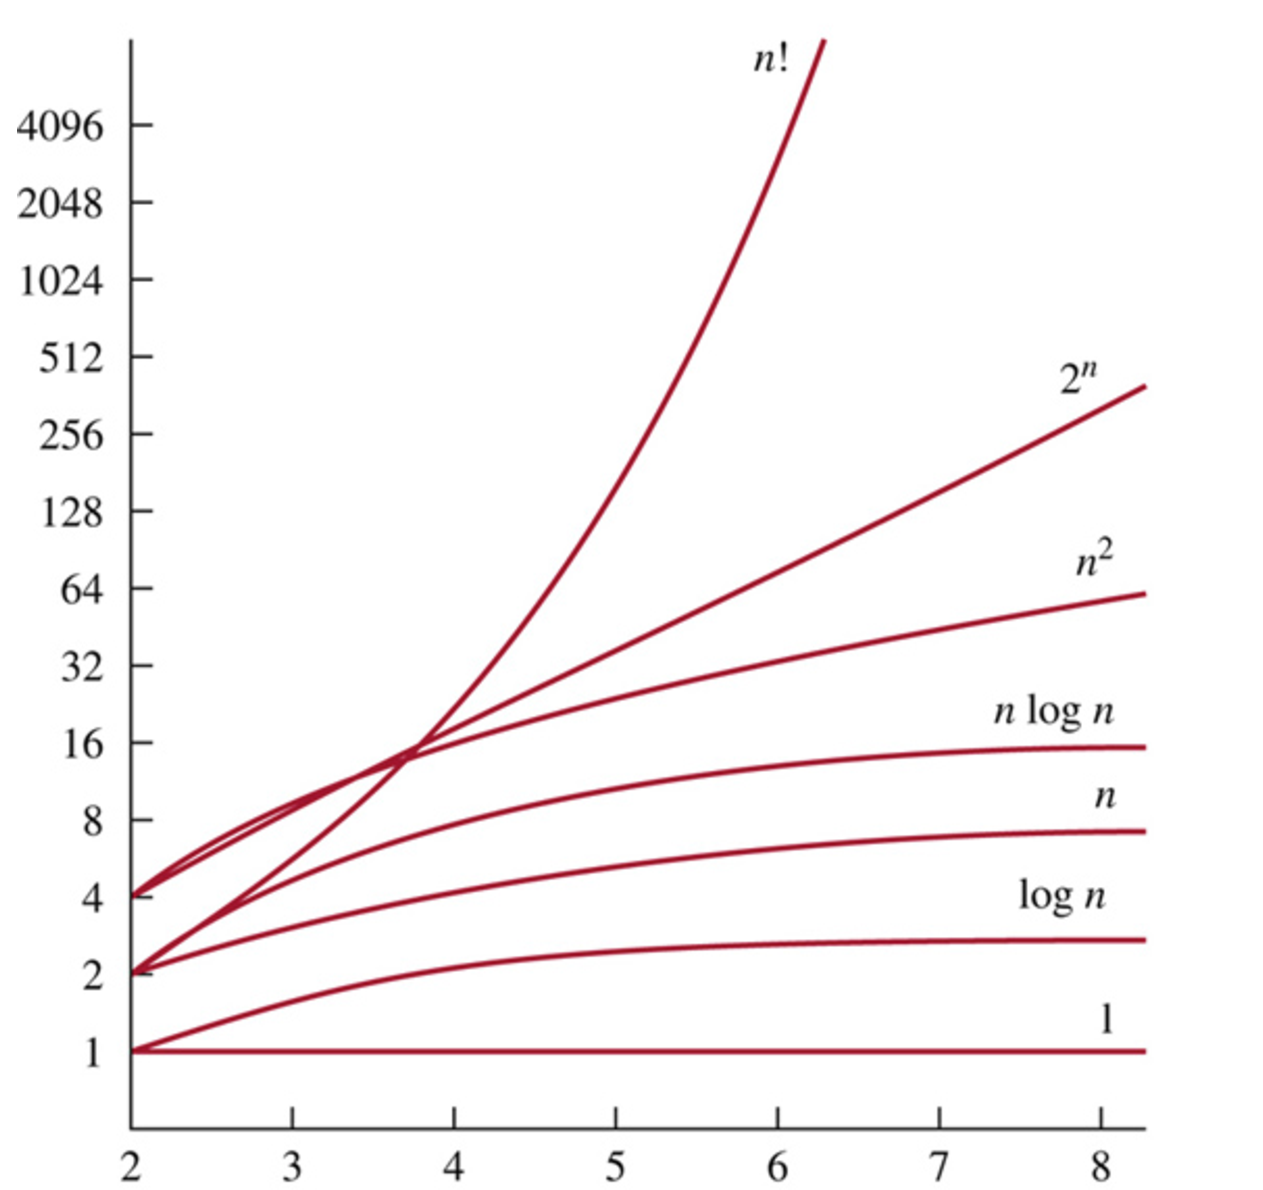
\includegraphics[width=0.4\linewidth]{images/laufzeiten}
	\caption{Laufzeiten}
\end{figure}

\subsection{Summenformel}
\paragraph{n Iterationen}
\begin{align}
	\frac{n \cdot (n + 1)}{2}
\end{align}

\subsection{n - 1 Iterationen}
\begin{align}
	\frac{n \cdot (n - 1)}{2}
\end{align}

\subsection{Stirling Formel}
\label{eq:stirling}
Die Stirling Formel kann für das Laufzeitverhalten von binären Suchbäumen verwendet werden.
\begin{align}
	\lim\limits_{n \rightarrow \infty} \log_2(n!) = n\cdot \log_2(n)
\end{align}

\section{Übersicht Datenstrukturen}
\begin{table}[h]
	\centering
	\begin{tabu} to \linewidth {X X c}
		\toprule
		Datenstruktur & Operationen & Laufzeitverhalten \\
		\midrule
		Array & get, set,   & $\mathcal{O}(1)$  \\
		Array & add, remove & $\mathcal{O}(n)$  \\
		List & addFirst, addLast, remove & $\mathcal{O}(1)$  \\
		List & get, set, add & $\mathcal{O}(n)$  \\
		Heap & Insert, remove, Up/Downheap & $\mathcal{O}(log(n))$  \\
		Heap & size, isEmpty, min, removeMin & $\mathcal{O}(1)$\\
		Map & put, get, remove & $\mathcal{O}(n)$ \\
		Map & Sentinel-Trick & halb so viele Abfragen \\
		Stack (Array-basiert) & alle Operationen & $\mathcal{O}(1)$ \\
		Stack (Array-basiert) & Speicherplatz & $\mathcal{O}(n)$ \\
		Deque & alle & $\mathcal{O}(1)$ \\
		Priority Queue & mit sortierter Liste & insert $\mathcal{O}(1)$, removeMin/min $\mathcal{O}(n)$\\
		Priority Queue & mit sortierter Liste & insert $\mathcal{O}(n)$, removeMin/min $\mathcal{O}(1)$\\
		Positional List mit doubly Linked List & suche nach pos & $\mathcal{O}(n)$ \\
		Positional List mit doubly Linked List & alle Operatione mit pos & $\mathcal{O}(1)$ \\
		Hash Table & Worst case (Kollisionen) & seach, insert, remove $\mathcal{O}(n)$ \\
		Hash Table & Gute Streuung & alle $\mathcal{O}(1)$ \\
		Skip List & search, remove, insert, height & $\mathcal{O}(log(n))$ \\
		Skip List & Speicherplatz & $\mathcal{O}(n)$ \\
		\bottomrule
	\end{tabu}
	\caption{Laufzeitverhalten von Datenstrukturen}
\end{table}

\subsection{Sortier- und Suchalgorithmen}
Weitere Sortieralgorithmen sind in Abschnitt \ref{sec:sortalgorithms} zu finden:
\begin{table}[h!]
	\centering
	\begin{tabu} to \linewidth {l l c c}
		\toprule
		Algorithmus & Datenstruktur & Best Case  & Worst Case\\
		\midrule
		Insertion Sort & Array & $\mathcal{O}(n^2)$ & $\mathcal{O}(n^2)$  \\
		Insertion Sort & Doubly-Linked List & $\mathcal{O}(n)$ & $\mathcal{O}(n^2)$  \\
		Insertion Sort & Priority Queue & $\mathcal{O}(n)$ & $\mathcal{O}(n^2)$  \\
		Selection Sort & Array & $\mathcal{O}(n^2)$ & $\mathcal{O}(n^2)$ \\
		Selection Sort & Doubly-Linked List & $\mathcal{O}(n^2)$ & $\mathcal{O}(n^2)$ \\
		Selection Sort & Priority Queue & $\mathcal{O}(n^2)$ & $\mathcal{O}(n^2)$ \\
		Heap Sort & Heap & $\mathcal{O}(n \cdot log(n))$ & $\mathcal{O}(n \cdot log(n))$ \\
		Linear Search & & $\mathcal{O}(n)$ & $\mathcal{O}(2n)$ \\
		Binary Search & & $\mathcal{O}(n)$ & $\mathcal{O}(n + log(n))$ \\
		\bottomrule
	\end{tabu}
	\caption{Laufzeitverhalten von Sortier- und Suchalgorithmen}
\end{table}


\section{Multimaps}
\begin{itemize}
	\item Multimaps sind immer ungeordnet
	\item Multimaps können mehrere der gleichen Elemente erhalten.
\end{itemize}

\subsection{Operationen}
\begin{description}
	\item[find(key)] Liefert den Wert für den Key oder null
	\item[findAll(key)] Liefert eine iterierbare Collection mit allen Werten zum Key
	\item[insert(key, value)] Fügt einen neuen Wert zum Schlüssel k ein
	\item[remove(node)] Entfernt den kompletten Knoten
\end{description}

\subsection{Geordnete Multimap}
Bei der geordneten Multimap sind die Keys der grösse nach geordnet. Sie besitzt folgende zusätzlichen Operationen.
\begin{description}
	\item[first()] Liefert den ersten Eintrag
	\item[last()] Liefert den letzten Eintrag
	\item[successor(key)] Liefert einen Iterator mit allen Knoten deren Key grösser oder gleich dem gegebenen Key ist.
	\item[predecessor(key)]  Liefert einen Iterator mit allen Knoten deren Key kleiner oder gleich dem gegebenen Key ist.
\end{description}

\section{Bäume}
\subsection{Terminologie}
\begin{description}
	\item[k-Baum] Ein Baum mit k Kindknoten pro Node
	\item[Wurzel / Root] Elternknoten
	\item[Interner Knoten] Knoten mit min. einem Child
	\item[Externer Knoten / Blattknoten] Knoten ohne Childs:
	\item[Vorgängerknoten] Parent
	\item[Tiefe] Anzahl Vorgänger (nach oben) (Der Wurzel Knoten hat die Tiefe = 0)
	\item[Höhe] Anzahl Ebenen der Nachfolger (nach unten). Die Höhe gibt die Anzahl Ebenen des Baumes an. (Externe Knoten haben die Höhe 0)
	\item[Subtree] Baum aus einem Knoten und seinen Nachfolger
	\item[Siblings] Zwillingsknoten
\end{description}

\subsection{Traversierung}
Gestartet wird immer beim Root, aufgeschrieben wird aber nur gemäss der Euler Tour Traversierung. Dabei zeichnet man startend links vom Parent Node eine Umrandung um den ganzen Tree und zieht bei jedem Knoten einen Strich in eine bestimmte Richtung:
\begin{description}
	\item[Preorder / Strich nach Links] \hfill \\
	Ein Node wird vor seinen Nachfolgern besucht, wobei zuerst der linke Node und danach der rechte Node abgearbeitet wird. ($Parent Node \Rightarrow Left Node \Rightarrow Right Node$)
	\item[Postorder / Strich nach Rechts] \hfill \\
	Ein Node wird nach seinen Nachfolgern besucht ($Left Node \Rightarrow Right Node \Rightarrow Parent Node$).
	\item[Inorder / Strich nach Unten] \hfill \\
	Ein Knoten wird \textbf{nach} seinem linken Subtree und \textbf{vor} seinem rechten Subtree besucht.
	($Left Node \Rightarrow Parent Node \Rightarrow Right Node$)
	\item[Breath First / Level Traversierung] \hfill \\
	Es werden zuerst alle Nodes einer Ebenen besucht bevor man zu einer tieferen Ebenen voranschreitet. Die Nodes werden dabei von links nach rechts abgearbeitet.
\end{description}

\subsubsection{Laufzeit}
Alle Traversierungen laufen mit $\Theta(n)$ (Theta)

\subsubsection{Implementierungen}
\begin{lstlisting}[caption=Inorder Traversal]
public Collection<Entry<K, V>> inorder() {
	Collection<Entry<K, V>> inorderCollection = new LinkedList<>();
	inorder(root, inorderCollection);
	return inorderCollection;
}

protected void inorder(Node node, Collection<Entry<K, V>> inorderCollection) {
	if (node != null) {
		inorder(node.getLeftChild(), inorderCollection);
		inorderCollection.add(node.getEntry());
		inorder(node.getRightChild(), inorderCollection);
	}
}

\end{lstlisting}

\section{BST: Binäre Such Bäume}
\begin{itemize}
	\item Im Gegensatz zu herkömmlichen Datenstrukturen (Array, Linked-Lists) mit linearer Laufzeit, erlauben Binäre Suchbäume \textbf{logarithmische Laufzeiten}
	\item Die \textbf{Inorder Traversal} retourniert die Keys in \textbf{geordneter Folge}
	\item Ein BST kann mit einer Map oder Multimap implementiert sein. Im Falle einer Map wird die Value einfach überschrieben.
	\item Gegeben sind immer drei Knoten \textbf{u, v, w} wobei:
	\begin{itemize}
		\item v die Root für den Teilbaum ist
		\item u im linken Teilbaum von v ist (kleinerer oder gleicher Wert)
		\item w im rechten Teilbaum von v ist (grösserer Wert)
		\item und $key(u) \leq key(v) \leq key(w)$
	\end{itemize}
	\item Der binäre Such Baum ist ein binärer Baum, der die Keys in seinen internen Knoten speichert
	\item Die externen Knoten speichern keine Daten, nur die internen
	\item Man erkennt am einfachsten, ob ein BST nullterminiert ist oder über externe abschliessende Nodes verfügt, wenn man im Konstruktor die Initialisierung der beiden Variablen \lstinline|leftson| und \lstinline|rightson| überprüft. (=\lstinline|null|?)
\end{itemize}


\subsection{Speicherplatz, Laufzeiten}
Find, Insert und Remove benötigen $\mathcal{O}(h)$ (Höhe), wobei die Höhe h im Worst Case $\mathcal{O}(n)$ und im Best Case $\mathcal{O}(log(n))$ ist. Der Worst Case ist wenn die Elemente vorsortiert eingefügt werden
\begin{table}[h]
	\centering
	\begin{tabu} to \linewidth {l l l}
		\toprule
		Methode & Best Case  & Worst Case \\
		\midrule
		Speicherplatz & $\mathcal{O}(n)$ & $\mathcal{O}(n)$ \\
		find() & $\mathcal{O}(log(n))$ &  $\mathcal{O}(n)$ \\
		insert() & $\mathcal{O}(log(n))$ & $\mathcal{O}(n)$ \\
		remove() & $\mathcal{O}(log(n))$ & $\mathcal{O}(n)$ \\
		sort()  & $\mathcal{O}(n\log(n))$ & $\mathcal{O}(n^2)$ \\
		\bottomrule
	\end{tabu}
	\caption{Laufzeitverhalten von Suchtabellen}
\end{table}

\subsection{Binäre Suche}
Binäre Suche benötigt immer random access, damit in die Mitte des Payloads springen kann und von dort aus die Suche starten kann. (\gls{gls-divideandconquer}) Des Weiteren müssen die Daten sortiert sein. Die binäre Suche ist eine Suche nach ''Einschachtelung'', da die linke und rechte Grenze immer enger zusammengezogen wird, bis man auf das Resultat stösst. Ein Suchpfad ist dann invalid, wenn eine der Grenzen überschritten wird.

\clearpage

\subsection{Operationen}
\begin{description}
	\item[find(key)] \hfill
	Liefert den Eintrag zum Schlüssel k oder null
	\begin{algorithm}
		\begin{algorithmic}[1]
			\IF{$T.isExternal(v)$}
			\RETURN{$null$}
			\ENDIF
			\IF{$k < key(v)$}
			\RETURN{$TreeSearch(k, T.left(v))$}
			\ELSIF{$k = key(v)$}
			\RETURN{$v$}
			\ELSE
			\RETURN$TreeSearch(k, T.right(v))$
			\ENDIF
		\end{algorithmic}
		\caption{TreeSearch(k,v)}
	\end{algorithm}
	\item[insert(key, object)] \hfill
	\begin{itemize}
		\item Wenn der Key noch nicht vorhanden ist, wird gemäss Binary Search Algorithm nach einem passenden Blatt Knoten gesucht. Wurde der Blatt Knoten gefunden, wird der neue Key eingefügt und in einen internen Knoten expandiert.
		\item Wenn der Key bereits vorhanden ist, wird ausgehend von dem ersten Treffer des existierenden Key im linken Teilbaum weitergesucht bis man auf einen passenden Blatt Knoten trifft. Wurde der Blatt Knoten gefunden, wird der neue Key eingefügt und in einen internen Knoten expandiert.
		\item Wenn man eine Multimap verwendet, werden mehrfache Knoten immer im linken Teilbaum eingefügt.
	\end{itemize}
	\begin{figure}[ht!]
		\centering
		\begin{minipage}[t]{0.4\textwidth}
			\centering
			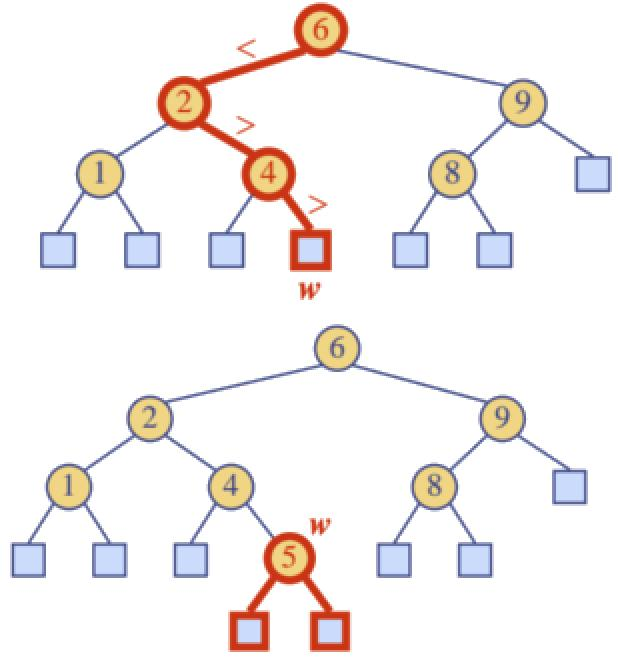
\includegraphics[width=0.9\linewidth]{images/search_tree_insert_1}
			\caption{Einfügen wenn der Key 5 noch nicht vorhanden}
			\label{fig:searchtreeinsert1}
		\end{minipage}
		\begin{minipage}[t]{0.4\textwidth}
			\centering
			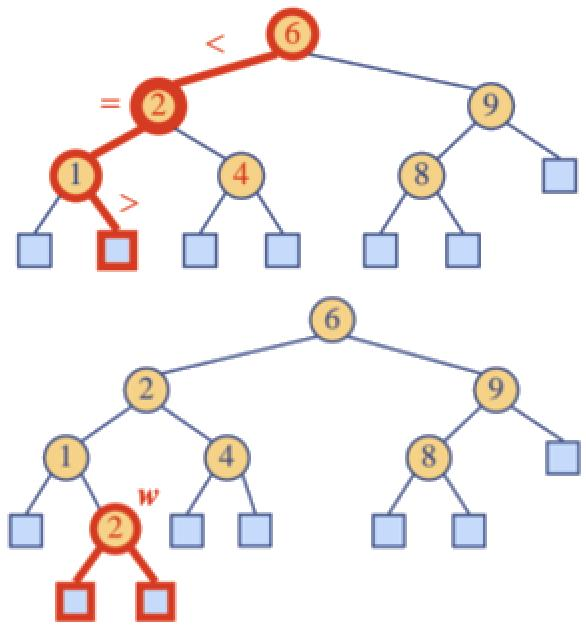
\includegraphics[width=0.9\linewidth]{images/search_tree_insert_2}
			\caption{Einfügen wenn der Key 2 bereits vorhanden}
			\label{fig:searchtreeinsert2}
		\end{minipage}
	\end{figure}
	
	\clearpage

	\begin{lstlisting}[caption=Arraylist basierter Einsatz]
	public void add(int lower, int upper, int content) {
		int middle = (lower + upper) / 2;
		if (content < arrayList.get(middle).intValue()) {
			// go left
			if (middle == 0 || content > arrayList.get(middle - 1)) {
				arrayList.add(middle, content);
			} else {
				add(lower, middle - 1, content);
			}
		} else {
			// go right
			if (middle + 1 >= arrayList.size() || content < arrayList.get(middle + 1)) {
				arrayList.add(middle + 1, content);
			} else {
			add(middle + 1, upper, content);
			}
		}
	}
	\end{lstlisting}

\clearpage

	\item[remove(key)] \hfill
	\label{sec:bstremove}
	\begin{itemize}
		\item Beim Löschen muss die Inorder Traversierung erhalten bleiben
		\item Beim Remove kann es vorkommen, dass gleiche Keys im linken und rechten Teilbaum der Root zu liegen kommen. Dies muss dann bei der Suche beachtet werden.
		\item Es wird zwischen drei Varianten unterschieden:
		\begin{itemize}
			\item Zu löschender Knoten hat \textbf{zwei Blatt Kinder}: \lstinline|removeExternal(w)| löscht den Blattknoten w und seinen Parent und ersetzt den Parent mit dem Geschwisterknoten von w
			\item Zu löschender Knoten hat \textbf{ein Blatt Kind}: Genau gleich wie beider Vorgehensweise mit zwei Blatt Kinder, jedoch mit dem Unterschied, dass der neue ''Parent'' kein Blattknoten ist.
			\item Zu löschender Knoten hat \textbf{keine Blatt Kinder}:  Man nimmt den nächsten Knoten in der Inorder Traversierung und ersetzt den zu löschen Key mit diesem. Der Key der kopiert wurde wird dann gelöscht.
		\end{itemize}
		\begin{figure}[ht!]
			\centering
			\begin{minipage}[t]{0.4\textwidth}
				\centering
				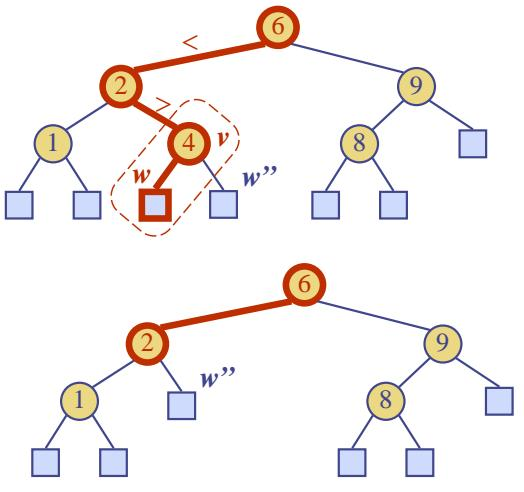
\includegraphics[width=0.9\linewidth]{images/search_tree_delete_1}
				\caption{Zwei Blatt Kinder}
				\label{fig:searchtreeinsert1}
			\end{minipage}
			\begin{minipage}[t]{0.4\textwidth}
				\centering
				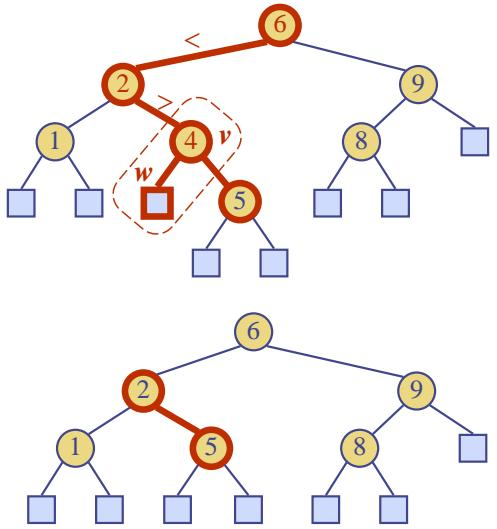
\includegraphics[width=0.9\linewidth]{images/search_tree_delete_2}
				\caption{Ein Blatt Kind}
				\label{fig:searchtreeinsert2}
			\end{minipage}
			\begin{minipage}[t]{0.4\textwidth}
				\centering
				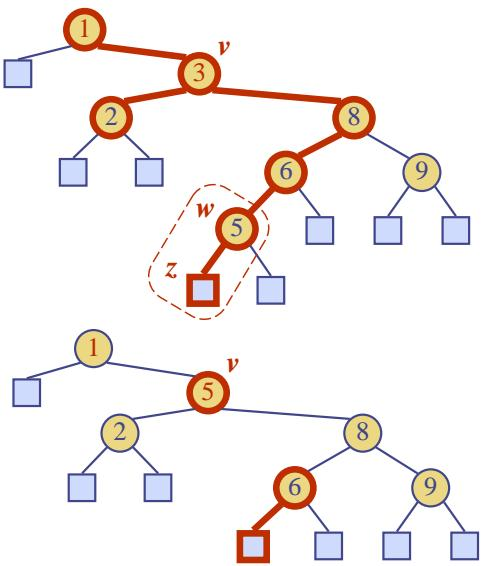
\includegraphics[width=0.9\linewidth]{images/search_tree_delete_3}
				\caption{Keine Blatt Kinder}
				\label{fig:searchtreeinsert1}
			\end{minipage}
		\end{figure}
	\end{itemize}
\end{description}
\clearpage

\subsection{Binäre Sortierung}
Eine Menge von n Zahlen kann sortiert werden, indem man diese zunächst in einen binären Suchbaum einfügt und dann durch das Inorder Traversal in sortierter Reihenfolge wieder ausgeben lässt.


\subsection{Speicherverbrauch}
Binäre Suchbäume haben folgenden Speicherverbrauch
\begin{table}[h]
	\centering
	\begin{tabu} to \linewidth {l l}
		\toprule
		Beschreibung & Big Oh \\
		\midrule
		Speicherverbrauch & $\mathcal{O}(n)$  \\
		Höhe & $\mathcal{O}(log(n))$ im besten Fall \\
		& $\mathcal{O}(n)$ im schlechtesten Fall \\
		\bottomrule
	\end{tabu}
	\caption{Speicherverbrauch von Binären Suchbäumen}
\end{table}

\subsection{Implementierungen}
\begin{lstlisting}[caption=BST Node]
public class Node {
	private Entry<K, V> entry;
	private Node leftChild;
	private Node rightChild;

	Node(int key) {
		this.key = key;
	}

	public Entry<K, V> setEntry(Entry<K, V> entry) {
		Entry<K, V> oldEntry = entry;
		this.entry = entry;
		return oldEntry;
	}
}
\end{lstlisting}

\begin{lstlisting}[caption=BST Entry]
public static class Entry<K, V> {
	private K key;
	private V value;

	protected K setKey(K key) {
		K oldKey = this.key;
		this.key = key;
		return oldKey;
	}

	public V setValue(V value) {
		V oldValue = this.value;
		this.value = value;
		return oldValue;
	}
}
\end{lstlisting}

\begin{lstlisting}
protected class RemoveResult {
	private Node node;
	private Entry<K, V> entry;
}
\end{lstlisting}



\begin{lstlisting}
public class BinarySearchTree<K extends Comparable<? super K>, V> {
	// Root node
	Node root;
	public BinarySearchTree() {
		root = null;
	}
	protected Node newNode(Entry<K, V> entry) {
		return new Node(entry);
	}
	public Entry<K, V> insert(K key, V value) {
		Entry<K, V> newEntry = new Entry<K, V>(key, value);
		root = insert(root, newEntry);
		return newEntry;
	}
	protected Node insert(Node node, Entry<K, V> entry) {
		if (node == null) {
			return newNode(entry);
		} else if (entry.getKey().compareTo(node.getEntry().getKey()) <= 0) {
			node.leftChild = insert(node.leftChild, entry);
		} else if (entry.key > node.key) {
			node.rightChild = insert(node.rightChild, entry);
		}
		return node;
	}
	public Entry<K, V> find(K key) {
		Node result = find(root, key);
		if (result == null) {
			return null;
		} else {
			return result.getEntry();
		}
	}
	protected Node find(Node node, K key) {
		if (node == null) {
			return null;
		}
		if (key.compareTo(node.getEntry().getKey()) < 0) {
			return find(node.leftChild, key);
		}
		if (key.compareTo(node.getEntry().getKey()) > 0) {
			return find(node.rightChild, key);
		}
		return node;
	};
	public Collection<Entry<K, V>> findAll(K key) {
		Collection<Entry<K, V>> entries = new LinkedList<Entry<K, V>>();
		findAll(root, key, entries);
		return entries;
	}

	protected void findAll(Node node, K key, Collection<Entry<K, V>> entries) {
		if (node == null) {
			return;
		}
		if (key.compareTo(node.getEntry().getKey()) == 0) {
			entries.add(node.getEntry());
		}
		if (key.compareTo(node.getEntry().getKey()) <= 0) {
			findAll(node.leftChild, key, entries);
		}
		if (key.compareTo(node.getEntry().getKey()) >= 0) {
			findAll(node.rightChild, key, entries);
		}
	}

	public Collection<Entry<K, V>> inorder() {
		Collection<Entry<K, V>> coll = new LinkedList<>();
		inorder(root, coll);
		return coll;
	}

	public Collection<Entry<K, V>> inorder() {
		Collection<Entry<K, V>> coll = new LinkedList<>();
		inorder(root, coll);
		return coll;
	}

	protected void inorder(Node node, Collection<Entry<K, V>> coll) {
		if (node == null) {
			return;
		}
		inorder(node.getLeftChild(), coll);
		coll.add(node.getEntry());
		inorder(node.getRightChild(), coll);
	}

	public Entry<K, V> remove(Entry<K, V> entry) {
		if (entry == null) {
			return null;
		}
		RemoveResult result = remove(root, entry);
		root = result.node;
		return result.entry;
	}

	protected RemoveResult remove(final Node node, final Entry<K, V> entry) {
		RemoveResult result = null;
		if (node == null) {
			return new RemoveResult(null, null);
		}
		if (entry.getKey().compareTo(node.getEntry().getKey()) < 0) {
			result = remove(node.leftChild, entry);
			node.leftChild = result.node;
			return result.set(node);
		} else if (entry.getKey().compareTo(node.getEntry().getKey()) > 0) {
			result = remove(node.rightChild, entry);
			node.rightChild = result.node;
			return result.set(node);
		} else {
			// Key found: is this the correct entry?
			if (node.getEntry() != entry) {
				// Searching for next entry with this key
				result = remove(node.leftChild, entry);
				node.leftChild = result.node;
				if (result.entry == null) {
					result = remove(node.rightChild, entry);
					node.rightChild = result.node;
				}
				return result.set(node);
			}
			// We have reachted the correct node.
			if (node.leftChild == null) {
				return new RemoveResult(node.rightChild, node.getEntry());
			}
			if (node.rightChild == null) {
				return new RemoveResult(node.leftChild, node.getEntry());
			}
			Entry<K, V> entryRemoved = node.getEntry();
			Node q = getParentNext(node);
			if (q == node) {
				node.setEntry(node.rightChild.getEntry());
				q.rightChild = q.rightChild.rightChild;
			} else {
				node.setEntry(q.leftChild.getEntry());
				q.leftChild = q.leftChild.rightChild;
			}
			return new RemoveResult(node, entryRemoved);
		}
	}

	protected Node getParentNext(Node p) {
		if (p.rightChild.leftChild != null) {
			p = p.rightChild;
			while (p.leftChild.leftChild != null) {
				p = p.leftChild;
			}
		}
		return p;
	}

	public int getHeight() {
		return getHeight(root);
	}

	protected int getHeight(Node parent) {
		if (parent == null) {
			return -1;
		} else {
			int leftHeight = getHeight(parent.leftChild);
			int rightHeight = getHeight(parent.rightChild);
			return Integer.max(leftHeight, rightHeight);
		}
	}

	public int size() {
		return size(root);
	}

	protected int size(Node n) {
		if (n == null) {
			return 0;
		}
		return size(n.leftChild) + size(n.rightChild) + 1;
	}

	public boolean isEmpty() {
		return size() == 0;
	}
}
\end{lstlisting}


\section{AVL Tree}
\begin{itemize}
	\item AVL Bäume sind BST die immer balanciert sind! (selbstbalanciert)
	\item Für jeden internen Knoten: Die Höhe darf sich bei beiden Kind Teilbäume um \textbf{höchstens um 1 unterscheiden}. (AVL Eigenschaft)
	\item Man spricht von der \textbf{Balance = Höhe(links) - Höhe(rechts)}. Die Balance darf somit -1, 0 oder 1 sein.
	\item Die Höhe ist immer $\mathcal{O}(log(n))$
	\item Die maximale (und mittlere) Anzahl Vergleiche, die nötig sind, um einen Schlüssel zu finden, hängt direkt mit der Höhe zusammen
	\item Er wurden von \gls{avl} erfunden
\end{itemize}

\subsection{Laufzeiten}
\begin{table}[h]
	\centering
	\begin{tabu} to \linewidth {l l}
		\toprule
		Methode & Best und Worst Case \\
		\midrule
		find() & $\mathcal{O}(log(n))$   \\
		insert() & $\mathcal{O}(log(n))$ \\
		remove() & $\mathcal{O}(log(n))$ \\
		rebalance() & $\mathcal{O}(log(n))$   \\
		\bottomrule
	\end{tabu}
	\caption{Laufzeitverhalten von AVL Trees}
\end{table}

\clearpage

\subsection{Operationen}
\paragraph{insert()}
Wenn der AVL Tree nach dem Einfügen unbalanciert ist, sucht man aufwärts in Richtung root, bis zum dem Knoten x, dessen Grosseltern (2 Ebenen höher) ein unbalancierten Knoten ist. Durch die \textbf{Trinode Umstrukturierung} (Siehe weiter unten) kann der AVL Tree wieder ausbalanciert werden
\begin{enumerate}
	\item x ist der gefundene Knoten
	\item y ist der parent des gefundenen Knoten
	\item z ist der grandparent des gefunden Knoten und der \textbf{Knoten der die AVL Eigenschaft verletzt}!
	\item Für x,y,z die Inorder Reihenfolge erstellen $\rightarrow$ (a,b,c)
	\item Baum \textbf{rotieren} gemäss a,b,c Anordnung
	\begin{itemize}
		\item LL: a zuunterst (schlägt nach links aus) $\rightarrow$ Rechts rotieren (b wird parent)
		\item RR: c zuunterst (schlägt nach rechts aus) $\rightarrow$ Links rotieren (b wird parent)
		\item LR: b zuunterst (hat Richtungswechsel links) $\rightarrow$ Doppelrotation rechts, links (b wird parent)
		\item RL: b zuunterst (hat Richtungswechsel rechts) $\rightarrow$ Doppelrotation links, rechts (b wird parent)
	\end{itemize}
\end{enumerate}
\paragraph{remove()} 
\begin{itemize}
	\item Das Löschen funktioniert wie beim BST. (Siehe \ref{sec:bstremove}) Ist der AVL Tree nach dem Löschen unbalanciert, muss er wieder in die Balance gebracht werden. Dazu müssen zuerst die Knoten identifiziert werden:
	\begin{itemize}
		\item z ist der erste unbalancierter Knoten
		\item y ist das Kind von z mit der \textbf{grösseren Höhe} als sein Sibling
		\item x ist das Kind von y mit der \textbf{grösseren Höhe} als sein Sibling
	\end{itemize} 
	\item Die Umstrukturierung kann eine neue Unbalance hervorrufen bei höheren Knoten im Baum. Somit muss die Balance weiter geprüft werden bis die Wurzel erreicht ist.
\end{itemize}

\clearpage

\subsection{Rotationen / Trinode Umstrukturierung}
Es gibt vier Varianten von Rotationen. Nach jeder Rotation muss die Inorder Traversal gleich bleiben!
\begin{lstlisting}[caption=AVL Tree Rotations]
protected AVLNode restructure(AVLNode xPos) {
	AVLNode yPos = xPos.getParent();
	AVLNode zPos = yPos.getParent();
	AVLNode newSubTreeRoot = null;
	if (yPos == zPos.getLeftChild()) {
		if (xPos == yPos.getLeftChild()) {
			newSubTreeRoot = rotateWithLeftChild(zPos);
		} else {
			newSubTreeRoot = doubleRotateWithLeftChild(zPos);
		}
	} else {
		if (xPos == yPos.getRightChild()) {
			newSubTreeRoot = rotateWithRightChild(zPos);
		} else {
			newSubTreeRoot = doubleRotateWithRightChild(zPos);
		}
	}
	return newSubTreeRoot;
}
\end{lstlisting}

\subsubsection{Rechts rotieren (einfach)}
Man rotiert auf die rechte Seite, wenn der Baum nach links schlägt (a zuunterst).
\begin{figure}[h!]
	\centering
	\begin{minipage}[t]{0.4\textwidth}
		\centering
		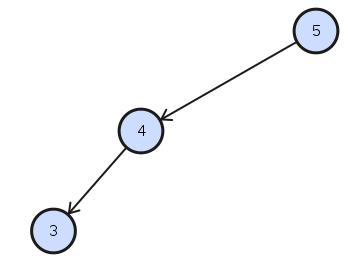
\includegraphics[width=0.7\linewidth]{images/avl_right_rotation_1}
		\caption{Rechts Rotation um c}
		\label{fig:trieexample}
	\end{minipage}
	\begin{minipage}[t]{0.4\textwidth}
		\centering
		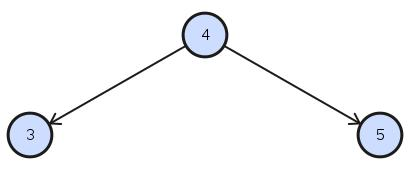
\includegraphics[width=0.9\linewidth]{images/avl_rotation_final}
		\caption{Nach der rechts Rotation}
		\label{fig:searchtreeinsert2}
	\end{minipage}
\end{figure}


\begin{lstlisting}[caption=AVL Tree: Single right rotation]
protected AVLNode rotateWithLeftChild(AVLNode k2) {
	AVLNode k1 = k2.getLeftChild();
	k2.setLeftChild(k1.getRightChild());
	k1.setRightChild(k2);

	if (k2.getLeftChild() != null) {
		k2.getLeftChild().setParent(k2);
	}
	adjustParents(k2, k1);

	return k1;
}
\end{lstlisting}

\subsubsection{Links rotieren (einfach)}
Man rotiert auf die linke Seite, wenn der Baum nach rechts schlägt (c zuunterst).
\begin{figure}[h!]
	\centering
	\begin{minipage}[t]{0.4\textwidth}
		\centering
		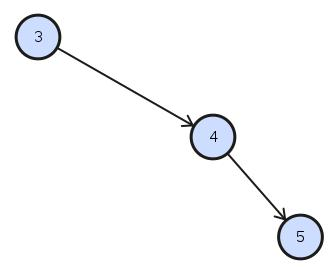
\includegraphics[width=0.7\linewidth]{images/avl_left_rotation_1}
		\caption{Links Rotation um a}
		\label{fig:trieexample}
	\end{minipage}
	\begin{minipage}[t]{0.4\textwidth}
		\centering
		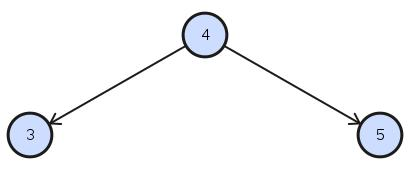
\includegraphics[width=0.9\linewidth]{images/avl_rotation_final}
		\caption{Nach der Links Rotation}
		\label{fig:searchtreeinsert2}
	\end{minipage}
\end{figure}

\begin{lstlisting}[caption=AVL Tree: Single left rotation]
protected AVLNode rotateWithRightChild(AVLNode k1) {
	AVLNode k2 = k1.getRightChild();
	k1.setRightChild(k2.getLeftChild());
	k2.setLeftChild(k1);

	if (k1.getRightChild() != null) {
		k1.getRightChild().setParent(k1);
	}
	adjustParents(k1, k2);
	
	return k2;
}
\end{lstlisting}

\clearpage

\subsubsection{Rechts/Links Doppelrotation}
Man rotiert zuerst nach rechts und dann nach links, wenn man einen Knick auf die linke Seite hat. (b zuunterst)
\begin{figure}[h!]
	\centering
	\begin{minipage}[t]{0.4\textwidth}
		\centering
		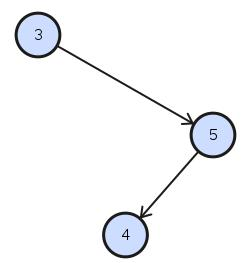
\includegraphics[width=0.7\linewidth]{images/avl_rightleft_rotation_1}
		\caption{Rechts Rotation um b}
		\label{fig:trieexample}
	\end{minipage}
	\begin{minipage}[t]{0.4\textwidth}
		\centering
		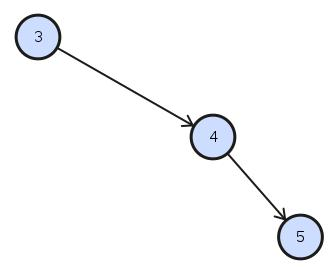
\includegraphics[width=0.9\linewidth]{images/avl_left_rotation_1}
		\caption{Links Rotation um a}
		\label{fig:searchtreeinsert2}
	\end{minipage}
	\begin{minipage}[t]{0.4\textwidth}
		\centering
		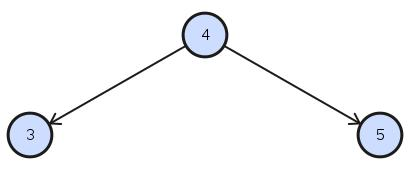
\includegraphics[width=0.9\linewidth]{images/avl_rotation_final}
		\caption{Nach Rechts/Links Rotation}
		\label{fig:searchtreeinsert2}
	\end{minipage}
\end{figure}
\begin{lstlisting}[caption=AVL Tree: Right/Left Rotation]
protected AVLNode doubleRotateWithLeftChild(AVLNode k3) {
	AVLNode rotatedRight = rotateWithRightChild(k3.getLeftChild());
	k3.setLeftChild(rotatedRight);
	return rotateWithLeftChild(k3);
}
\end{lstlisting}

\clearpage

\subsubsection{Links/Rechts Doppelrotation}
Man rotiert zuerst nach links und dann nach rechts, wenn man einen Knick auf die rechte Seite hat. (b zuunterst)
\begin{figure}[h!]
	\centering
	\begin{minipage}[t]{0.4\textwidth}
		\centering
		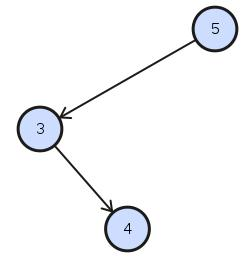
\includegraphics[width=0.7\linewidth]{images/avl_leftright_rotation_1.jpg}
		\caption{Links Rotation um a}
		\label{fig:trieexample}
	\end{minipage}
	\begin{minipage}[t]{0.4\textwidth}
		\centering
		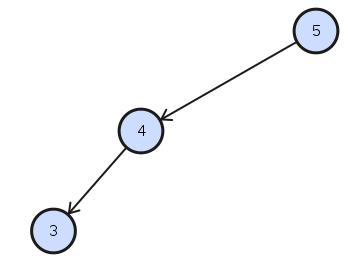
\includegraphics[width=0.9\linewidth]{images/avl_right_rotation_1}
		\caption{Rechts Rotation um c}
		\label{fig:searchtreeinsert2}
	\end{minipage}
	\begin{minipage}[t]{0.4\textwidth}
		\centering
		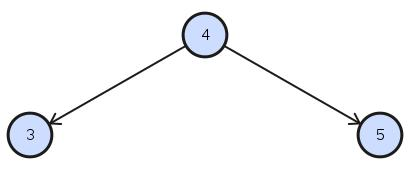
\includegraphics[width=0.9\linewidth]{images/avl_rotation_final}
		\caption{Nach Links/Rechts Rotation}
		\label{fig:searchtreeinsert2}
	\end{minipage}
\end{figure}
\begin{lstlisting}[caption=AVL Tree: Left/Right Rotation]
protected AVLNode doubleRotateWithRightChild(AVLNode k3) {
	AVLNode rotatedLeft = rotateWithLeftChild(k3.getRightChild());
	k3.setRightChild(rotatedLeft);
	return rotateWithRightChild(k3);
}
\end{lstlisting}

\clearpage

\subsection{Cut/Link Restrukturierung}
Die Cut/Link Restrukturierung bewirkt das selbe wie die Rotationen. Er ist zwar komplexer, dafür eleganter, da man keine Fallunterscheidung machen muss. Die Laufzeit ist aber gleich wie bei den Rotationen.
\begin{enumerate}
	\item Wie bei den Rotation muss zuerst x,y,z und a,b,c identifiziert werden
	\begin{enumerate}
		\item x ist der gefundene Knoten
		\item y ist der parent des gefundenen Knoten
		\item z ist der grandparent des gefunden Knoten und der \textbf{Knoten der die AVL Eigenschaft verletzt}!
		\item Für x,y,z die Inorder Reihenfolge erstellen $\rightarrow$ (a,b,c)
	\end{enumerate}
	\item Identifiiziere die Subtrees T0, T1, T2, T3 (Inorder Traversierung) von a,b und c
	\item Aufschreiben des Inorder Arrays (1-7) $\rightarrow$ Inorder Reihenfolge
	\begin{table}[h]
		\centering
		\begin{tabu} to \linewidth {| c | c | c | c | l | l | l |}
			\toprule
			$T_0$ & a & $T_1$ & b & $T_2$ & c & $T_3$ \\ \hline
			1 & 2 & 3 & 4 & 5 & 6 & 7 \\
			\bottomrule
		\end{tabu}
		\caption{Inorder Array für Cut/Link Restrukturierung}
	\end{table}
	\item Setze a als linkes Kind von b
	\item Setze c als rechtes Kind von b
	\item Setze T0 als linken und  T1 als rechten Unterbaum von a
	\item Setze T2 als linken  und T3 als rechten Unterbaum von c.
\end{enumerate}


\begin{figure}[h]
\centering
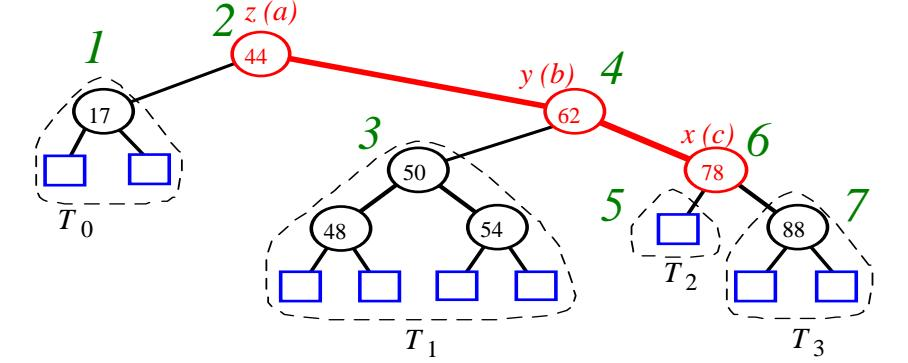
\includegraphics[width=0.8\linewidth]{images/cut_link_restruction}
\caption{Cut/Link Restrukturierung}
\label{fig:cutlinkrestruction}
\end{figure}

\begin{figure}[h]
	\centering
	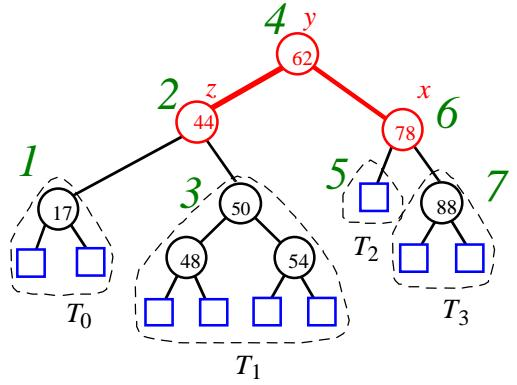
\includegraphics[width=0.6\linewidth]{images/cut_link_restruction_solution}
	\caption{Balancierter Baum nach Cut/Link}
	\label{fig:cutlinkrestructionsolution}
\end{figure}



\subsection{Implementierung}
\begin{lstlisting}[caption=AVL Tree Node]
protected class AVLNode extends BinarySearchTree<K, V>.Node {
	private int height;
	private Node parent;

	AVLNode(Entry<K, V> entry) {
		super(entry);
	}

	protected AVLNode setParent(AVLNode parent) {
		AVLNode old = avlNode(this.parent);
		this.parent = parent;
		return old;
	}

	protected int setHeight(int height) {
		int old = this.height;
		this.height = height;
		return old;
	}

	protected AVLNode getParent() { .. }
	protected int setHeight() { .. }


	@Override
	public AVLNode getLeftChild() {
		return avlNode(super.getLeftChild());
	}

	@Override
	public AVLNode getRightChild() {
		return avlNode(super.getRightChild());
	}
}
\end{lstlisting}

\begin{lstlisting}[caption=AVL Tree]
class AVLTreeImpl<K extends Comparable<? super K>, V> extends BinarySearchTree<K, V> {

	protected AVLNode actionNode;

	protected AVLNode getRoot() {
		return avlNode(root);
	}

	protected AVLNode avlNode(Node node) {
		return (AVLNode) node;
	}

	public int getHeight() {
		return height(avlNode(root));
	}

	protected int height(AVLNode node) {
		return (node != null) ? node.getHeight() : -1;
	}

	public V put(K key, V value) {
		Entry<K, V> entry = super.find(key);
		if (entry != null) {
			// key already exists in the Tree
			return entry.setValue(value);
		} else {
			// key does not exist in the Tree yet
			super.insert(key, value);
			rebalance(actionNode);
			actionNode = null;
			return null;
		}
	}

	public V get(K key) {
		Entry<K, V> entry = super.find(key);
		if (entry != null) {
			return entry.getValue();
		} else {
			return null;
		}
	}

	@Override
	protected Node insert(Node node, Entry<K, V> entry) {
		if (node != null) {
			actionNode = avlNode(node);
		}
		// calling now the BST-insert() which will do the work:
		AVLNode result = avlNode(super.insert(node, entry));
		if (node == null) {
			// In this case: result of super.insert() is the new node!
			result.setParent(actionNode);
		}
		return result;
	}

	protected Node newNode(Entry<K, V> entry) {
		AVLNode avlNode = new AVLNode(entry);
		return avlNode;
	}

	public V remove(K key) {
		Entry<K, V> entry = super.find(key);

		Entry<K, V> toReturn = super.remove(entry);
		if (toReturn == null) {
			AVLNode zPos = actionNode;
			rebalance(zPos);
		}
		return toReturn.getValue();
	}

	protected boolean isBalanced(AVLNode node) {
		int leftHeight = height(node.getLeftChild());
		int rightHeight = height(node.getRightChild());

		int balance = leftHeight - rightHeight;
		return (balance >= -1) && (balance <= 1);
	}

	protected void rebalance(AVLNode node) {
		while (node != null) {
			setHeight(node);
			if (!isBalanced(node)) {
				AVLNode xPos = tallerChild(tallerChild(node));
				node = restructure(xPos);
				setHeight(node.getLeftChild());
				setHeight(node.getRightChild());
				setHeight(node);
			}
			node = node.getParent();
		}
	}

	protected AVLNode tallerChild(AVLNode node) {
		AVLNode leftChild = node.getLeftChild();
		AVLNode rightChild = node.getRightChild();
		if (height(leftChild) >= height(rightChild)) {
			return leftChild;
		} else {
			return rightChild;
		}
	}

	protected void setHeight(AVLNode node) {
		if (node == null) {
			return;
		}

		int heightLeftChild = -1;
		if (node.getLeftChild() != null) {
			heightLeftChild = node.getLeftChild().getHeight();
		}

		int heightRightChild = -1;
		if (node.getRightChild(); != null) {
			heightRightChild = node.getRightChild();.getHeight();
		}

		node.setHeight(1 + Math.max(heightLeftChild, heightRightChild));
	}

	protected void adjustParents(final AVLNode oldSubtreeRoot, final AVLNode newSubtreeRoot) {
		final AVLNode parentSubtree = oldSubtreeRoot.getParent();
		oldSubtreeRoot.setParent(newSubtreeRoot);
		if (oldSubtreeRoot == root) {
			newSubtreeRoot.setParent(null);
			root = newSubtreeRoot;
		} else {
			newSubtreeRoot.setParent(parentSubtree);
			if (oldSubtreeRoot == parentSubtree.getLeftChild()) {
				parentSubtree.setLeftChild(newSubtreeRoot);
			} else {
				parentSubtree.setRightChild(newSubtreeRoot);
			}
		}
	}

	protected void inorder(Collection<AVLNode> nodeList, AVLNode node) {
	if (node == null)
	return;
	inorder(nodeList, node.getLeftChild());
	nodeList.add(node);
	inorder(nodeList, node.getRightChild());
	}
}
\end{lstlisting}

\section{Splay Tree}
\begin{itemize}
	\item Splay Trees sind auch binäre Suchbäume mit der zusätzlichen Operation \lstinline|splay()|. Dies verschiebt den gefundenen Knoten in die Root.
	\item Das spezielle an Splay Trees ist es, dass sie nach jeder Operation (auch bei der Suche) dem Baum rotiert wird. Die Rotation ist dieselbe wie bei AVL Trees.
	\item Oft verwendete Elemente sind somit immer nahe beim Root und können schnell zugegriffen werden! (z.B bei Suchmaschinen, Caching, Garbage Collection)
	\item Das Bewegen eines Knoten zur Root unter Benutzung von Rotationen nennt man Splaying
	\begin{itemize}
		\item \textbf{Zig:} linkes Kind (rechtsrotation)
		\item \textbf{Zag:} rechtes Kind (linksrotation)
	\end{itemize}
	\item Die Rotation hängt davon ab, welcher Typ von Kind x ist (links-rechts, rechts-rechts, etc.) z.B Ist x das linke Kind von seinem Parent, welcher selber ein rechtes Kind von seinem Parent ist (x = links-rechts Grosskind) $\rightarrow$ \textbf{Immer ausgehend von x!}
	\item Der Knoten x wird nach einem Zugriff zur Root bewegt (nach Update und Suchen)
\end{itemize}

\subsection{Varianten}
\begin{figure}[h]
\centering
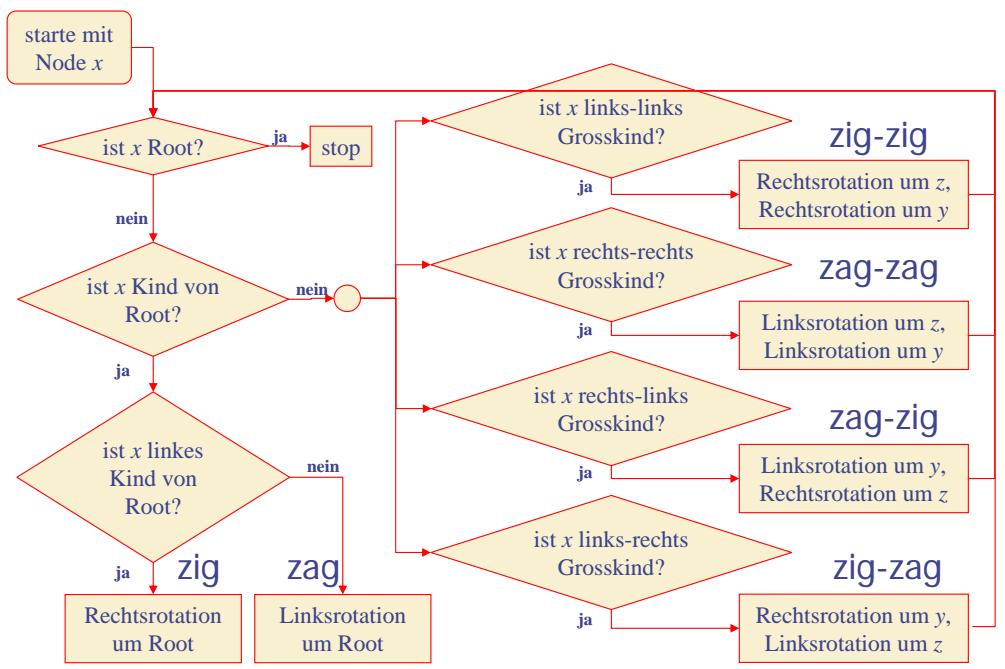
\includegraphics[width=0.9\linewidth]{images/splay_tree_flow_diagram}
\caption{Splay Tree Flussdiagramm}
\label{fig:splaytreeflowdiagram}
\end{figure}

\subsection{Vorgehen}
\begin{enumerate}
	\item Knoten identifizieren
	\begin{enumerate}
		\item x ist der gesuchte/eingefügte Knoten (Spezialfall löschen)
		\item y ist der Parent von x
		\item z ist der Parent von y
	\end{enumerate}
	\item Gemäss Flussdiagramm korrekte Fall auswählen und Rotation durchführen.
\end{enumerate}

\begin{figure}[h]
	\centering
	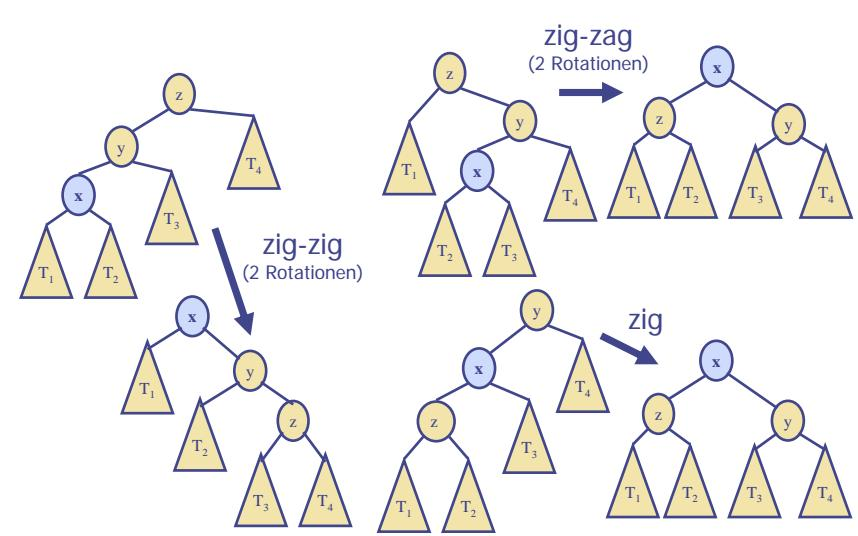
\includegraphics[width=0.7\linewidth]{images/splay_trees_zig-zag}
	\caption{Splay Tree Beispiele}
	\label{fig:splaytreeszig-zag}
\end{figure}

\subsection{Remove}
Beim Löschen wir der zu löschende Knoten mit dem nächsten Knoten in der \textbf{Inorder Reihenfolge} ersetzt.Man sieht am folgenden Beispiel, wobei der Wert 8 gelöscht wird.
\begin{enumerate}
	\item Ersetze zu löschenden Knoten mit seinem Inorder Nachfolder. Dies ist nicht immer möglich, z.B wenn der zu löschende Knoten in externer Knoten ist. In diesem Fall kann dieser Schritt ausgelassen werden
	\item Identifiziere x,y,z
	\begin{itemize}
		\item x = Parent vom löschenden Knoten
		\item y = Parent von x
		\item z = Parent von z
	\end{itemize}
	\item Lösche den zu löschenden Knoten
	\item Rotiere gemäss Zig-Zag Schema, damit x in die Root kommt.
\end{enumerate}

\begin{figure}[h!]
	\centering
	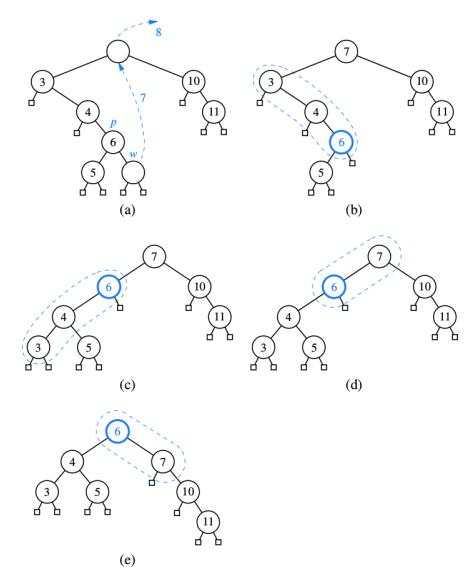
\includegraphics[width=0.5\linewidth]{images/splay_trees_remove}
	\caption{Splay Tree: Löschen des Wert 8}
	\label{fig:splaytreesremove}
\end{figure}

\newpage


\subsection{Splaying}
Bei den Operationen werden jeweils andere Knoten gesplayed. Ziel jeder Operation ist es, dass der betroffenen Knoten immer als Root gesetzt wird. Dabei wird der zu findende/löschende Knoten x genannt.
\begin{table}[h!]
	\centering
	\begin{tabu} to \linewidth {l l}
		\toprule
		Methode & Knoten zum Splayen \\
		\midrule
		find(k) & wenn der Key gefunden, benutze diesen Knoten \\
		 & wenn Key nicht gefunden, benutzen den Parent des externen Knoten am Ende \\
		 insert(k, v) & Benutze den neuen Knoten bei welchem der Entry eingefügt/ersetzt wurde \\
		 remove(k) & Benutze den Parent des internen Knotens welcher gelöscht wurde. \\
		\bottomrule
	\end{tabu}
	\caption{Laufzeitverhalten von Splay Trees}
\end{table}


\subsection{Laufzeiten}
\begin{table}[h!]
\centering
	\begin{tabu} to \linewidth {l l l}
	\toprule
	Methode & Laufzeitverhalten  & Beschreibung\\
	\midrule
	splay() & $\mathcal{O}(h) \rightarrow \mathcal{O}(n)$  & h=Height, Worst Case \\
	 & $\mathcal{O}(log(n))$ & Durchschnitt\\
	\bottomrule
	\end{tabu}
	\caption{Laufzeitverhalten von Splay Trees}
\end{table}

\section{Sortieralgorithmen} \label{sec:sortalgorithms}
\subsection{Eigenschaften}
\begin{description}
	\item[inplace] \hfill \\
	Ein Algorithmus arbeitet inplace, wenn er nur den Speicherplatz für die Input Daten benötigt und zusätzlich nur konstanten (\textbf{vom Input unabhängige} Menge an Speicher) verwendet. Der Algorithmus überschreibt also die Eingabedaten mit den Ausgabedaten.	
	\item[stabil]  \hfill \\
	Die relative Ordnung von zwei Items mit dem selben Key werden durch den Algorithmus nicht verändert. Die Ordnung bleibt in der Zielsequenz erhalten. (z.B wichtig bei Bestellungen vom selben Kunden. Die Reihenfolge muss erhalten bleiben)
\end{description}

\subsection{Varianten}
\begin{description}
	\item[Vergleichsbasierte Sortieralgorithmen] Vergleichsbasierte Algorithmen basieren auf dem paarweisen Vergleich der zu sortierenden Elemente. Bei der Komplexitätsanalyse wird davon ausgegangen, dass der Aufwand zum Vergleich zweier Elemente konstant ist.
	\item[Nicht vergleichsbasierte Sortieralgorithmen] Bei Sortierverfahren, die nicht auf Vergleichen beruhen, kann ein linearer Anstieg der benötigten Zeit mit der Anzahl der zu sortierenden Elemente erreicht werden. Bei großen Anzahlen zu sortierender Datensätze sind diese Algorithmen \textbf{den vergleichsbasierten Verfahren überlegen}, sofern sie (wegen des \textbf{zusätzlichen Speicherbedarfs}) angewendet werden können. Zudem können sie allerdings nur für numerische Datentypen verwendet werden.
\end{description}

\subsection{Laufzeiten}
Die untere Grenze aller folgenden Algorithmen kann mit der Stirling Formel (\ref{eq:stirling}) hergeleitet werden. Vergleichsbasierte Algorithmen wie Bubble Sort, Selection Sort, Insertion Sort, Heap Sort, Merge Sort, Quick Sort haben eine minimale Laufzeit von $\Omega(n \cdot log(n))$ (\textbf{Untere Grenze})
\begin{table}[h]
	\centering
	\begin{tabu} to \linewidth {l l X}
		\toprule
		Algorithmus & Big Oh & Bemerkung \\
		\midrule
		Selection Sort & $\mathcal{O}(n^2)$ & langsam, \textbf{in-place}, für kleine Daten Sets (< 1K) \\
		Insertion Sort & $\mathcal{O}(n^2)$ & langsam, \textbf{in-place}, \textbf{stable}, für kleine Daten Sets (< 1K) \\
		Heap Sort & $\mathcal{O}(n \cdot log(n))$ & schnell, \textbf{in-place}, für grosse Daten Sets (1K - 1M) \\
		Merge Sort & $\mathcal{O}(n \cdot log(n))$ & schnell, \textbf{stable} sequentieller Datenzugriff, für riesige Data Sets (> 1M) \\
		Quick Sort & $\mathcal{O}(n \cdot log(n))$ & schnellster, \textbf{in-place}, (typischweise nicht stable)\\
		\bottomrule
	\end{tabu}
	\caption{Laufzeitverhalten von vergleichbasierten Sortieralgorithmen}
\end{table}

\begin{table}[h]
	\centering
	\begin{tabu} to \linewidth {l l X}
		\toprule
		Algorithmus & Big Oh & Bemerkung \\
		\midrule
		Bucket Sort & $\mathcal{O}(n + N)$ & Nur für positive Ganzzahlen \\
		Radix Sort & $\mathcal{O}(d \cdot (n+N))$ &  d = Anzahl Tupel, N = Max Key Bereich \\
		\bottomrule
	\end{tabu}
	\caption{Laufzeitverhalten von nicht vergleichbasierten Sortieralgorithmen}
\end{table}


\subsection{Lexikographische Sortierung}
\begin{itemize}
	\item Ein Tupel ist ein Satz von Werten der i-ten Ordnung (3 Tupel = kartesische Koordinaten im Raum)
	\item Für die Lexikographische Sortierung ist ein Comparator nötig, der zwei Tupel nach ihrer i-ten Dimension vergleicht
	\item Für Lexikographische Sortierung ist ebenfalls ein stabiler Sortieralgorithmus nötig
	\item Lexikografische Sortierung läuft mit $\mathcal{O}(n \cdot \mathcal{S}(n))$, wobei $\mathcal{S}(n)$ der Laufzeit des stabilen Sortieralgorithmus darstellt.
\end{itemize}

\begin{algorithm}[h!]
	\KwData{sequence S of d-Tuples}
	\KwResult{sequence S sorted in lexicographic order}
	
	\For{$i \leftarrow d$ \textbf{downto} 1}
	{
		stableSort(S, $C_i$)
		
	}
	\caption{lexicographicSort(S)}
\end{algorithm}


\begin{figure}[h!]
	\centering
	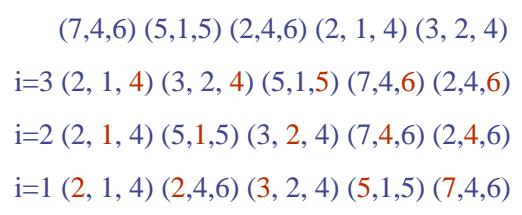
\includegraphics[width=0.7\linewidth]{images/lexikographic_sort}
	\caption{Lexikographische Sortierung}
	\label{fig:lexikographicsort}
\end{figure}


\section{Bubble Sort}
\begin{itemize}
	\item Der Bubble Sort ist ein sehr trivialer Sortieralgorithmus
	\item Er loopt über eine Sequenz und vertauscht ein Item mit dem Nächsten, falls dieses grösser als das Nächste ist. Die wird solange wiederholt, bis keine Vertauschungen stattgefunden haben.
	\item Ist stabil
\end{itemize}
\subsection{Laufzeiten}
\begin{table}[h]
	\centering
	\begin{tabu} to \linewidth {l l X}
		\toprule
		Big Oh & Beschreibung & Bemerkung \\
		\midrule
		Best Case & $\mathcal{O}(n)$ & Aufsteigend sortierte Sequnez (1 Iteration, n Vergleiche) \\
		Worst Case & $\mathcal{O}(n^2)$ & Absteigend sortierte Sequenz (n Iterationen, n Vergleiche) \\
		Worst Case mit Optimierung & $\mathcal{O}(n^2)$ & Absteigend sortierte Sequenz (n - 1 Iterationen, n - i Vergleiche) \\
		\bottomrule
	\end{tabu}
	\caption{Big Oh Merge Sort}
\end{table}

\begin{lstlisting}[caption=Bubble Sort]
public static <T extends Comparable<? super T>> void bubbleSort2(T[] sequence) {
	// performance improvement -> last item is always sorted after iteration
	int max = sequence.length;
	boolean sorted = false;
	do {
		boolean swapped = false;
		for (int i = 1; i < sequence.length; i++) {
			if (sequence[i].compareTo(sequence[i - 1]) < 0) {
				T temp = sequence[i];
				sequence[i] = sequence[i - 1];
				sequence[i - 1] = temp;
				swapped = true;
			}
		}

		max--;

		if (!swapped) {
			sorted = true;
		}

	} while(!sorted);
}
\end{lstlisting}


\section{Merge Sort}
\begin{itemize}
	\item Merge Sort basiert auf \textbf{Divide and Conquer}
	\item Läuft mit $\mathcal{O}(n \cdot log(n))$ (gleich wie der Heap Sort)
	\item Die Verankerung der Rekursion ist immer ein Teilproblem der grösse 0 oder 1
	\item Merge Sort wird von Java für die Sortierung verwendet. (Für die Sortierung von primitven Typen wird QuickSort verwendet.)
	\item Im Gegensatz zum Quicksort finden die Vergleiche beim Merge Sort während dem Rücklauf der Rekursion ab.
	\item Ist \textbf{stable} aber nicht in-place
	\item Ist meist langsamer wie Quick Sort.
\end{itemize}

\subsection{Laufzeiten}
\begin{table}[h]
	\centering
	\begin{tabu} to \linewidth {l l}
		\toprule
		Big Oh & Beschreibung \\
		\midrule
		Höhe & $\mathcal{O}(log (n))$ \\
		Laufzeit Sortieren & $\mathcal{O}(n \cdot log(n))$ \\
		\bottomrule
	\end{tabu}
	\caption{Big Oh Merge Sort}
\end{table}

\clearpage

\begin{lstlisting}[caption=Nicht Rekursiver Merge Sort]
public static void mergeSort(Object[] orig, Comparator c) {

	Object[] in = new Object[orig.length];

	// make a new temporary array
	System.arraycopy(orig,0,in,0,in.length);

	// copy the input
	Obj ect[] out = new Obj ect[in.length]; // output array
	Obj ect[] temp; // temp array reference used for swapping.
	int n = in.length;

	// each iteration sorts all length-2*i runs
	for (int i=1; i < n; i*=2) {

		// each iteration merges two length-i pair
		for (int j=0; j  < n; j +=2*i)  {}
			// merge from in to out two length-i runs at j
			merge(in,out,c,j ,i);
		}

		// swap arrays for next iteration
		temp = in;
		in = out;
		out = temp;
	}
	// the "in" array contains the sorted array, so re-copy it
	System.arraycopy(in,0,orig,0,in.length);
}

protected static void merge(Object[] in, Object[] out, Comparator c, int start, int inc) {
	// merge in[start..start+inc-1] and
	// in[start+inc..start+2*inc-1]
	int x = start; // index into run # 1
	int end1 = Math.min(start+inc, in.length);

	// boundary for run # 1
	int end2 = Math.min(start+2*inc, in.length);

	// boundary for run # 2
	int y = start+inc;

	// index into run # 2 (could be beyond array boundary)
	int z = start; // index into the out array
	while ((x < end1) && (y < end2)) {
		if (c.compare(in[x],in[y]) <= 0) {
			out[z++] = in[x++];
		} else {
			out[z++] = in[y++];
		}
	}

	 // first run didn't finish
	if (x < end1) {
		System.arraycopy(in, x, out, z, end1 - x);
	} else if (y < end2) { // second run didn't finish
		System.arraycopy(in, y, out, z, end2 - y);
	}
}
\end{lstlisting}


 \section{Quick Sort}
\begin{itemize}
	\item Beim Quicksort wird die Menge in \textbf{drei Teile unterteilt (Divide)} 
	\begin{enumerate}
		\item \textbf{L}: Less: Alle Elemente kleiner x
		\item \textbf{E}: Pivot: Alle Elemente gleich x
		\item \textbf{G}: Greater: Alle Elemente grösser x
	\end{enumerate}
	\item \textbf{Recur}: Sortiere L und G
	\item \textbf{Conquer}: vereine L, E und G
	\item Es gibt verschiedenen Möglichkeiten um das \textbf{Pivot} zu wählen. (Oft zufällig, am besten der Median)
	\item Die Laufzeit hängt stark von der Wahl des Pivots ab. Er ist deshalb nicht geeignet für Realtime Applikationen. Wird das Pivot jedoch gut gewählt, ist der Algorithmus sehr schnell.
	\item Der Quick Sort Algorithmus ist typischerweise nicht stabil, da er mit Swap Operationen arbeitet. Es gibt stabile Varianten.
\end{itemize}

\subsection{Laufzeiten}
\begin{table}[h]
	\centering
	\begin{tabu} to \linewidth {l l X X}
		\toprule
		Big Oh & Beschreibung & Bemerkung & Anzahl Vergleiche \\
		\midrule
		Worst Case Laufzeit & $\mathcal{O}(n^2)$ & Wenn Pivot das Minimum oder Maximum ist & \\
		Best Case Laufzeit &  $\mathcal{O}(n \cdot log(n))$ & Wen das Pivot der Median & $\sum_{i=1}^{n-1} i = \frac{(n-1)n}{2}$\\
		Höhe & $\mathcal{O}(log(n))$ & \\
		\bottomrule
	\end{tabu}
	\caption{Big Oh Quick Sort}
\end{table}

\subsection{In Place Implementierung}
\begin{enumerate}
	\item Pivot x = 6
	\item Wiederholung bis h und k sich kreuzen
	\begin{enumerate}
		\item h nach rechts bis zu einem Element $\geq$ Pivot x
		\item k nach links bis zu einem Element $<$ Pivot 1x
		\item Wenn h und k noch nicht gekreuzt: Elemente mit Indizes h und k vertauschen
	\end{enumerate}
\end{enumerate}
\begin{figure}[h]
\centering
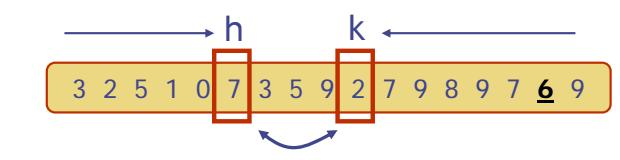
\includegraphics[width=0.35\linewidth]{images/quicksort_inplace}
\caption{InPlace Quicksort}
\label{fig:quicksortinplace}
\end{figure}

\newpage



\begin{lstlisting}[caption=Inplace Quick Sort]
public static void quickSort (Object[] S, Comparator c) {
	if (S.length < 2) {
		return; // the array is already sorted in this case
	}
	quickSortStep(S, c, 0, S.length-1); // recursive sort method
}

private static void quickSortStep (Object[] S, Comparator c, int leftBound, int rightBound ) {

	if (leftBound >= rightBound) {
		return; // the indices have crossed
	}

	Object temp;  // temp object used for swapping
	Object pivot = S[rightBound];
	int leftIndex = leftBound;     // will scan rightward
	int rightIndex = rightBound-1; // will scan leftward
	while (leftIndex <= rightIndex) {
		// scan right until larger than the pivot
		while ( (leftIndex <= rightIndex) && (c.compare(S[leftIndex], pivot)<=0) ) {
			leftIndex++;
		}

		// scan leftward to find an element smaller than the pivot
		while ( (rightIndex >= leftIndex) && (c.compare(S[rightIndex], pivot)>=0)) {
			rightIndex--;
		}


		// swap
		if (leftIndex < rightIndex) { // both elements were found
			temp = S[rightIndex];
			S[rightIndex] = S[leftIndex]; // swap these elements
			S[leftIndex] = temp;
		}
	} // the loop continues until the indices cross

	temp = S[rightBound]; // swap pivot with the element at leftIndex
	S[rightBound] = S[leftIndex];
	S[leftIndex] = temp; // the pivot is now at leftIndex, so recurse

	// step over equal elements to speed up
	while ((leftIndex > leftBound) && (comp.compare(sequence[leftIndex], sequence[leftIndex - 1]) == 0)) {
		leftIndex--;
	}
	while ((rightIndex > 0) && (rightIndex < rightBound) && (comp.compare(sequence[rightIndex], sequence[rightIndex + 1]) == 0)) {
		rightIndex++;
	}

	// recursive call
	quickSortStep(S, c, leftBound, leftIndex-1);
	quickSortStep(S, c, leftIndex+1, rightBound);
}

\end{lstlisting}

\section{Bucket Sort}
\begin{itemize}
	\item Bucket Sort funktioniert nur mit positven Ganzzahlen in einem Bereich
	\item Bucket Sort \textbf{ist stabil}
	\item S: Sequenz von n Items
	\item N: Maximaler Key
	\item n: Anzahl Items (Key, Value), mit Key im Bereich von [0, N-1]
	\item Der Bucket Sort benutzt die Keys als Index in einem Hilfs-Array B von Sequenzen
	\item Der Algorithmus ist in \textbf{drei Phasen eingeteilt}:
	\begin{enumerate}
		\item Partitionierung: Verteilung der Elemente auf die Buckets B[k]
		\item Jeder Bucket wird mit einem weiteren Sortierverfahren wie beispielsweise Insertionsort sortiert
		\item Der Inhalt der sortierten Buckets wird konkateniert
	\end{enumerate}
\end{itemize}

\begin{figure}[h]
\centering
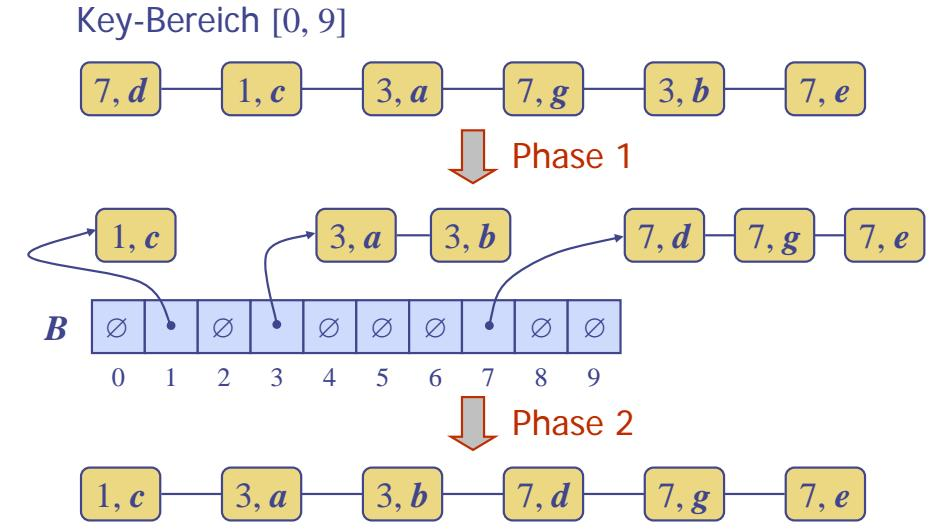
\includegraphics[width=0.8\linewidth]{images/bucketsort}
\caption{Bucket Sort}
\label{fig:bucketsort}
\end{figure}


\subsection{Laufzeiten}
\begin{table}[h]
	\centering
	\begin{tabu} to \linewidth {l l}
		\toprule
		Big Oh & Bemerkung \\
		\midrule
		$\mathcal{O}(n + N)$ & Nur für positive Ganzzahlen \\
		\bottomrule
	\end{tabu}
	\caption{Big Oh Bucket Sort}
\end{table}

\clearpage

\subsection{Implementierung}
\begin{lstlisting}
 public static void sort(int[] a, int maxVal) {
	 // fail fast
	 if (maxVal <= 0) {
		 throw new IllegalArgumentException();
	 }
	 if (a.length <= 1) {
		 return a; //trivially sorted
	 }
 
	 int[] bucket= new int[maxVal + 1];
	
	 for (int i=0; i<bucket.length; i++) {
		 bucket[i]=0;
	 }
	
	 // Phase 1:
	 for (int i=0; i<a.length; i++) {
		 bucket[a[i]]++;
	 }
	
	 // Phase 2: 
	 int outPos=0;
	 for (int i=0; i < bucket.length; i++) {
		 for (int j=0; j<bucket[i]; j++) {
			 a[outPos++]=i;
		 }
	 }
}
\end{lstlisting}

\clearpage


\section{Radix Sort}
\begin{itemize}
	\item Der Radix Sort ist eine Spezialisierung der lexikographischen Sortierung, welcher Bucket Sort als Sortieralgorithmus verwendet
	\item Er ist ebenfalls kein vergleichsbasierter Sortieralgorithmus wie z.B QuickSort, etc.
	\item Ist \textbf{stabil}
	\item Voraussgesetzt, dass die maximale Länge der zu sortierenden Schlüssel im vornherein bekannt sind, läuft Radix Sort mit linearer Laufzeit.
	\item Er besteht aus zwei Phasen:
	\begin{enumerate}
		\item \textbf{Partitionierungsphase}: In dieser Phase werden die Daten in die vorhandenen Fächer aufgeteilt, wobei für jedes Zeichen des zugrundeliegenden Alphabets ein Fach zur Verfügung steht
		\item \textbf{Sammelphase}: Nach der Aufteilung der Daten in Fächer in Phase 1 werden die Daten wieder eingesammelt und auf einen Stapel gelegt
	\end{enumerate}
\end{itemize}

\subsection{Laufzeiten}
\begin{table}[h]
	\centering
	\begin{tabu} to \linewidth {l l}
		\toprule
		Big Oh & Bemerkung \\
		\midrule
		$\mathcal{O}(d \cdot (n+N))$ & d = Anzahl Tupel, N = Key Bereich Max\\
		\bottomrule
	\end{tabu}
	\caption{Big Oh Bucket Sort}
\end{table}

\subsection{Beispiel}
Die Sequenz 124, 523, 483, 128, 923, 584 soll sortiert werden.
\begin{lstlisting}
// 1. partition: order by last digit
|0| |1| |2| |3| |4| |5| |6| |7| |8| |9|
				 |     |           	        |
			   523   124           		  128
			   483   584 
			   923
// 2. collect: 523, 483, 923, 124, 584, 128
// 3. partition: order by second digit
|0| |1| |2| |3| |4| |5| |6| |7| |8| |9|
		    |                               |
		   523                             483
		   923                             584
		   124
		   128
		
// 4. collect: 523, 923, 124, 128, 483, 584
// 5. partition: order by first digit
|0| |1| |2| |3| |4| |5| |6| |7| |8| |9|
	   |               |    |                    |
	   124             483  523                  923
	   128                  584

// 6. collect: 
124, 128, 483, 523, 584, 923
\end{lstlisting}

\clearpage

\subsection{Implementierung}
\begin{lstlisting}
public class RadixSort {
	// array of linked lists
	private final LinkedList<String>[] buckets;
	
	public RadixSort() {
		// create LinkedList for buckets
		buckets = (LinkedList<String>[]) new LinkedList<?>[1 + ('z' - 'a' + 1)];
		IntStream.range(0, buckets.length).forEach(
			i -> buckets[i] = new LinkedList<String>()
		);
	}

	public void radixSort(String[] data) {
	
		// find max index
		AtomicInteger maxLength = new AtomicInteger(-1);
		Arrays.stream(data).forEach(str -> {
			if (str.length() > maxLength.intValue()) {
				maxLength.set(str.length());
			}
		});
	
		// bucketsort from max index to first index
		for (int i = maxLength.get() - 1; i >= 0; i--) {
			bucketSort(data, i);
		}
	
	}
	
	protected void bucketSort(String[] data, int index) {
	
		// clear buckets
		Arrays.stream(buckets).forEach(list -> list.clear());
	
		// insert data elements to buckets
		Arrays.stream(data).forEach(str -> {
			if (str.length() <= index) {
				buckets[0].addLast(str);
			} else {
				buckets[str.charAt(index) - 'a' + 1].addLast(str);
			}
		});
	
		// shift bucket elements back into data array
		AtomicInteger i = new AtomicInteger(0);
		Arrays.stream(buckets).forEach(list -> list.forEach(str -> {
			data[i.getAndIncrement()] = str;
		}));
	}
}
\end{lstlisting}

\section{Pattern Matching}
\begin{description}
	\item[T] Der Text in dem gesucht werden soll
	\item[P] Ein String (Pattern)
	\item[m] Die Länge des Strings P
	\item[s] Länge des Alphabets $\Sigma$
	\item[i] Index im Text
	\item[j] Index im Pattern
	\item[Präfix] Substring vom Typ P[0 .. i]
	\item[Suffix] Substring vom Typ P[i .. (m-1)]
\end{description}

\subsection{Laufzeiten}
\begin{table}[h]
	\centering
	\begin{tabu} to \linewidth {l l X}
		\toprule
		Algorithmus & Big Oh & Bemerkung \\
		\midrule
		Brute Force Algorithmus & $\mathcal{O}(n \cdot m)$ & \\
		Boyer-Moore Algorithmus & $\mathcal{O}(n \cdot m + s)$ & Ist der schnellste (obschon schlechter Worst Case: Sogar schlechter wie Brute Force) \\
		Knuth-Morris-Pratt Algorithmus & $\mathcal{O}(n+m)$ & \\
		& $\mathcal{O}(n+m)$ (Fehlfunktion)\\
		\bottomrule
	\end{tabu}
	\caption{Big Pattern Matching Boyer-Moore und KMP}
\end{table}

\subsection{Brute Force Algorithmus}
Der Brute Force Algorithmus vergleicht das Pattern P mit dem Text T für jede mögliche Position.
\begin{algorithm}[H]
	\KwData{Text T der Länge n und Pattern P der Länge m}
	\KwResult{Startindex eines Substrings von T, welcher mit P übereinstimmt, oder -1 falls kein solcher Substring existiert}
	\For{$i \leftarrow 0$ \KwTo n - m}
	{
		$j \leftarrow 0$ \\
		\While{$j < m \land T[i+j] = P[j]$}{
			 $j \leftarrow j + 1$
		}

		\If{j = m} {
			\Return{i}
		}
	}
	\Return -1
\caption{BruteForceMatch(T, P)}
\end{algorithm}


\subsection{Boyer-Moore Algorithmus}
\begin{itemize}
	\item Benötigt $\mathcal{O}(n\cdot m + s)$
	\item Der Algorithmus startet mit den Vergleichen am \textbf{Ende des Pattern}
	\item Verwendet \textbf{Character Jump Heuristik}: Falls keine Übereinstimmung $\rightarrow$ Richte das Pattern gemäss dem letzten Mismatch Zeichen im Pattern aus
\end{itemize}

\subsubsection{Last Occurence Funktion}
Man erstellt eine Hashmap für alle Zeichen des Alphabets $\Sigma$ mit dem letzten Auftreten des Zeichens c im Pattern. Das neue i berechnet sich wie folgt:
\[
	i = i + m - min(j, (last(c) + 1))
\]
wobei
\begin{itemize}[label=]
	\item i = Index des Missmatch Character in Text T
	\item m = Länge des Patterns
	\item c = Alle möglichen Zeichen des Text Alphabets
	\item L(c) = Letztes Auftreten des Zeichens c im Pattern (Start bei Index 0) (-1, falls nicht vorhanden)
\end{itemize}

\begin{figure}[h]
\centering
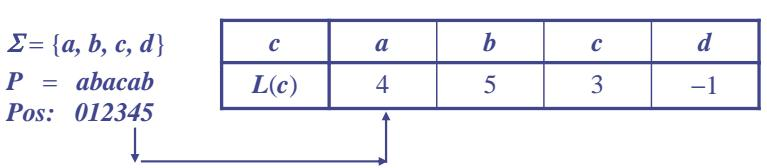
\includegraphics[width=0.9\linewidth]{images/boyer_moore_last_occurence}
\caption{Boyer Moore Last Occurence}
\label{fig:boyermoorelastoccurence}
\end{figure}

\clearpage

\subsubsection{Vorgehen}
\begin{enumerate}
	\item Erstelle die Last Occurence Funktion
	\item Starte am Ende des Patterns und Vergleiche das Pattern mit dem Text (\textbf{Rechts nach Links})
	\item Bei einem Missmatch, unterscheide folgende Fälle:
	\begin{enumerate}
		\item Wenn das Zeichen c \textbf{im Text} auch im Pattern vorkommt, verschiebe das Pattern bis zu dieser Stelle. (Siehe Last Funktion, falls Zeichen mehrmals vorhanden)
		\item Wenn das Zeichen c \textbf{im Text} auch im Pattern vorkommt, aber die Last Funktion einen Index zurückliefert, der der \textbf{grösser ist} wie der Index des Mismatches, verschiebe einfach um 1.
		\item Wenn das Zeichen c im Text nicht im Pattern vorkommt, verschiebe das Pattern um die Länge des Patttern.
	\end{enumerate}
\end{enumerate}

\begin{figure}[h]
	\centering
	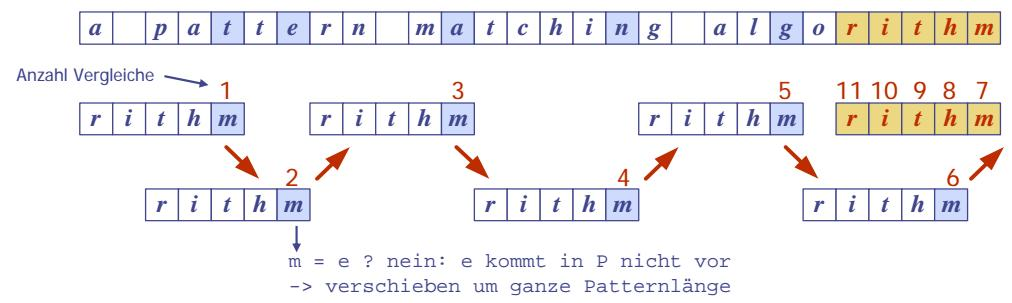
\includegraphics[width=0.9\linewidth]{images/boyer_moore_algorithm}
	\caption{Boyer Moore Algorithmus}
	\label{fig:boyermoorealgorithm}
\end{figure}

\subsubsection{Implementierung}
Gegeben ist der Text T, das Pattern P und das Alphabet. \hfill \\
\begin{algorithm}[H]
	$L \leftarrow lastOccurenceFunction(P, \Sigma)$ \\
	$i \leftarrow m -1$ \tcp{Index in T}
	$j \leftarrow m -1$ \tcp{Index in P}
	\Repeat{i > n -1}{
		\eIf{T[i] = P[j]}{
			\eIf{j=0} {
				\Return i \tcp{match}
			}
			{
				$i \leftarrow i - 1$ \\
				$j \leftarrow j - 1$
			}
		}
		{
			$l \leftarrow L[T[i]]$ \\
			$i \leftarrow i + m - min(j, 1 + l)$ \\
			$j \leftarrow m - 1$
		}

	}
	\Return -1
	\caption{BoyerMooreMatch(T, P, $\Sigma$)}
\end{algorithm}

\clearpage

\subsection{KMP: Knuth-Morris-Pratt Algorithmus}
Durch das Preprocessing beim KMP Algorithmus erreicht man eine Geschwindigkeit die \textbf{proportional zur Textlänge} ist.
\begin{itemize}
	\item Benötigt $\mathcal{O}(n + m)$
	\item Der Knut-Morris-Pratt Algorithmus vergleicht das Muster wie der Bruteforce von links nach rechts, aber schiebt das Muster intelligenter als dieser.
	\item Es wird um so viele Zeichen verschoben, sodass der \textbf{Präfix gleichzeitig auch Suffix} ist. Dies wird wie beim Boyer-Moore Algorithmus in einer Vorlaufsphase aufgebaut.
\end{itemize}

\subsubsection{Fehl-Funktion}
Die Fehlfunktion ist definiert als die Grösse des längsten Präfixes, sodass dieser auch Suffix des Patterns ist. Man betrachtet dabei immer einen Substring. Es sind auch Überlappungen (siehe Beispiel Index 6) möglich. Die Fehlfunktion läuft mit $\mathcal{O}(m)$

\begin{enumerate}
	\item Füge das Pattern in der zweiten Reihe der Tabelle ein
	\item Betrachte das Pattern Schritt für Schritt, wobei man immer mehr Zeichen anschaut. (bis zur maximalen Länge). Der Präfix startet immer ganz Links und der Suffix ended immer ganz rechts! Leserichtung ist immer von links nach rechts.
	\item Suche die maximale Länge für ein Pattern, das zugleich Präfix und Suffix ist. Es können auch Überschneidungen auftreten.
\end{enumerate}

\begin{figure}[h]
\centering
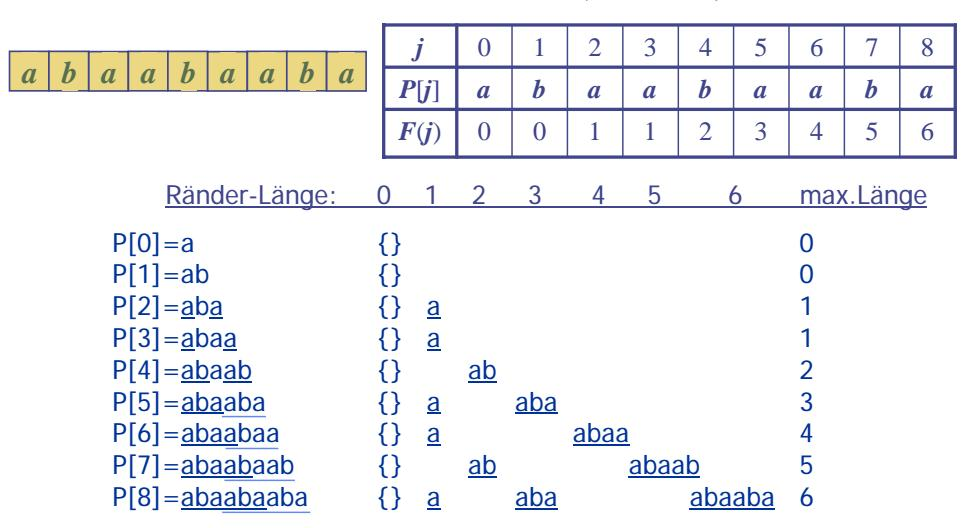
\includegraphics[width=0.9\linewidth]{images/fehlfunktion}
\caption{1. Fehlfunktion aufbauen}
\label{fig:fehlfunktion}
\end{figure}

\clearpage

\subsubsection{Vorgehen}
\begin{enumerate}
	\item Gehe von \textbf{Links nach Rechts}
	\item Suche den ersten Mismatch (j=5)
	\item Übergib die Stelle des \textbf{Zeichens davor} (j = (5 - 1) = 4) der Fehlfunktion F(4)
	\item Der Rückgabewert der Fehlfunktion (=1) ist dann das Zeichen (j = 1 $\rightarrow$ zweites b), welches bis zur Position des Missmatch vorgeschoben werden kann.
	\item Ist der Rückgabewert = 0 wird das Pattern einfach um 1 verschoben
\end{enumerate}


\begin{figure}[h]
\centering
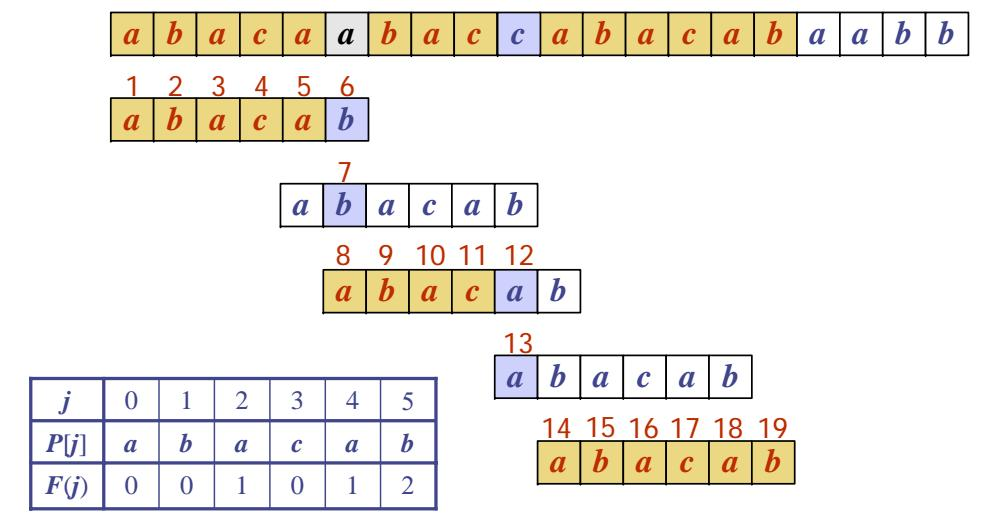
\includegraphics[width=0.8\linewidth]{images/kmp_match_algorithm}
\caption{2. Knuth-Morris-Pratt Algorithm}
\label{fig:kmpmatchalgorithm}
\end{figure}

\clearpage

\subsubsection{Implementierung}

\begin{lstlisting}[caption=Knuth-Morris-Pratt Algorithmus]
public static int KMPmatch(String text, String pattern) {
	int n = text.length();
	int m = pattern.length();
	int[] fail = computeFailFunction(pattern);
	printFail(fail);
	int i = 0;
	int j = 0;
	while (i < n) {
	System.out.print("\ni = " + i + " j = " + j);
		if (pattern.charAt(j) == text.charAt(i)) {
			if (j == m - 1) {
					return i - m + 1; // match
			}
			i++;
			j++;
		} else if (j > 0) {
			j = fail[j - 1];
		} else {
			i++;
		}
	}
	return -1; // no match
}
\end{lstlisting}


\begin{lstlisting}[caption=Knuth-Morris-Pratt Algorithmus Fehlfunktion]
public static int[] computeFailFunction(String pattern) {
	int[] fail = new int[pattern.length()];
	fail[0] = 0;
	int m = pattern.length();
	int j = 0;
	int i = 1;
	while (i < m) {
		if (pattern.charAt(j) == pattern.charAt(i)) {
			// j + 1 characters match
			fail[i] = j + 1;
			i++;
			j++;
		} else if (j > 0) {
			// j follows a matching prefix
			j = fail[j - 1];
	 	} else {
		 	// no match
			fail[i] = 0;
			i++;
		}
	}
	return fail;
}
\end{lstlisting}


\section{Tries}
\begin{itemize}
	\item Mit der Trie Datenstruktur ist ein Pattern Matching möglich, das \textbf{proportional zur Grösse des Pattern} ist. (im Vergleich zum KNP, der proportional zum Text läuft)
	\item Bei Tries gibt es ein Preprocessing des Textes so, dass die Wörter im Baum und die Position als Leaf gespeichert sind.
	\item \textbf{Gross/Kleinschreibung} muss beachtet werden, wobei grosse Buchstaben vor kleinen aufgelistet wird.
\end{itemize}

\subsection{Standard Trie}
\begin{itemize}
	\item Der Standard Trie ist ein geordneter Baum für eine Menge von Strings (S), so dass:
	\begin{itemize}
		\item jeder äussere Knoten ausser der Root hat die Kinder alphabetisch geordnet
		\item die Pfade von der Root zun den externen Knoten beinhalten die Wörter/Strings
	\end{itemize}
\end{itemize}

\subsubsection{Vorgehen}
\begin{enumerate}
	\item Root zeichnen (leerer Knoten)
	\item Root Childs für alle Anfangsbuchstaben erstellen und diese alphabetisch ordnen \\ (ACHTUNG: \textbf{Gross/Kleinschreibung beachten}: GROSS vor klein)
	\item Vorheriger Schritt wiederholen, bis alle Zeichen im Trie abgelegt sind.
	\item Jeder Blattknoten speichert die Positionen des assozierten Wortes.
\end{enumerate}

\begin{figure}[h]
\centering
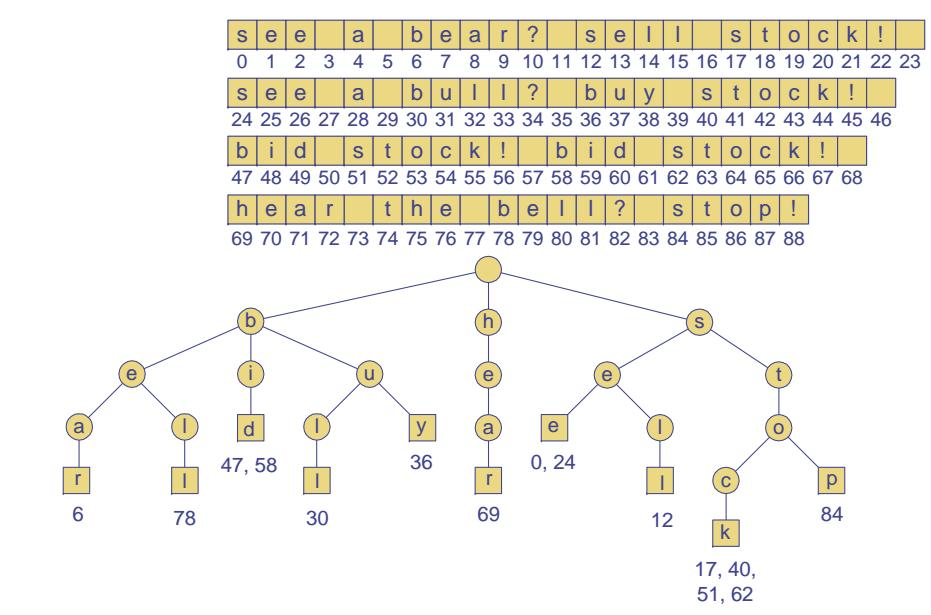
\includegraphics[width=0.8\linewidth]{images/trie_example}
\caption{Trie Beispiel}
\label{fig:trieexample}
\end{figure}


\subsection{Komprimierter Trie}
\begin{itemize}
	\item Beim komprimierten Trie haben alle \textbf{internen Knoten mindestens 2 Kinder} und nach Möglichkeit mehrere Buchstaben pro Node.
	\item Die kompakte Representation eines komprimierten Tries ist ein Array aller Strings
	\begin{itemize}
		\item Jeder Knoten speichert dann nur noch die Indizes in dem Array anstatt den Strings
		\item \lstinline|[index im array], [start zeichen innerhalb des array item] [end zeichen innerhalb des array item]|
		\item z.B \lstinline|S[3] = "stock"| $\rightarrow$ Knoten = (3,1,2) $\rightarrow$ \lstinline|"to"|
	\end{itemize}
\end{itemize}
\begin{figure}[ht!]
	\centering
	\begin{minipage}[t]{0.4\textwidth}
		\centering
		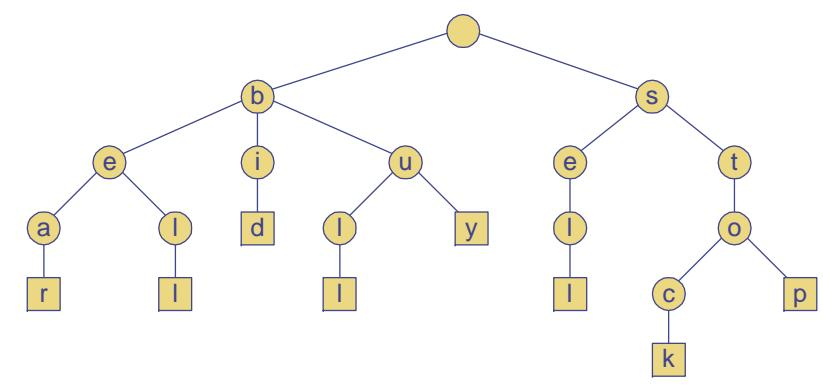
\includegraphics[width=0.9\linewidth]{images/compressed_trie_init}
		\caption{Trie Ausgangslage}
		\label{fig:trieexample}
	\end{minipage}
	\begin{minipage}[t]{0.4\textwidth}
		\centering
		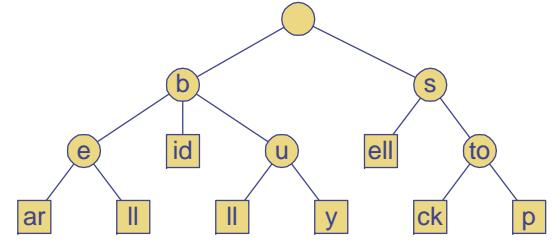
\includegraphics[width=0.9\linewidth]{images/compressed_trie}
		\caption{Trie nach Kompression}
		\label{fig:searchtreeinsert2}
	\end{minipage}
\end{figure}


\begin{figure}[h]
\centering
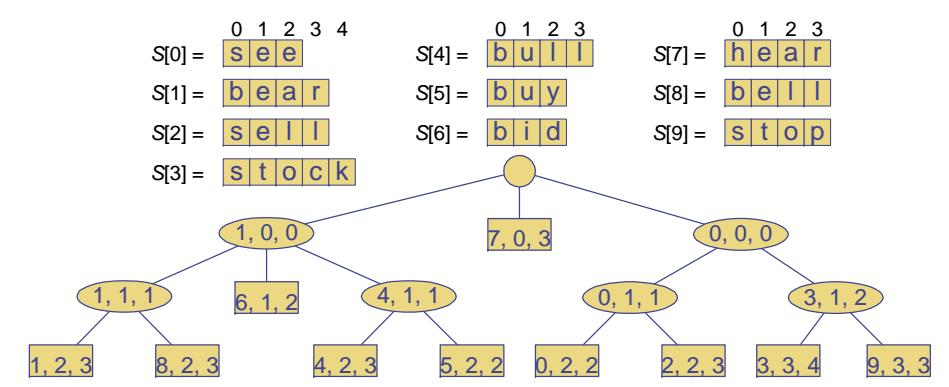
\includegraphics[width=0.7\linewidth]{images/compressed_trie_representation}
\caption{Kompakte Repräsentation eines komprimierten Tries}
\label{fig:compressedtrierepresentation}
\end{figure}

\subsection{Suffix Trie}
\begin{itemize}
	\item Der Suffix Trie eines Strings ist der komprimierte Trie von allen Suffixen des Strings
	\item Mit eine Suffix kann alles gefunden werden (nicht nur am Wortanfang)
	\begin{itemize}
		\item Das komplette Wort
		\item Suffix
		\item Prefix
		\item Substrings
	\end{itemize}
\end{itemize}
\begin{figure}[ht!]
	\centering
	\begin{minipage}[t]{0.4\textwidth}
		\centering
		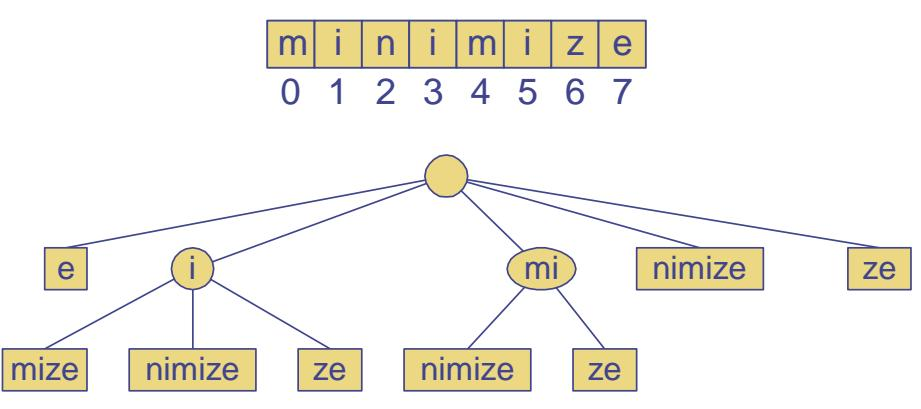
\includegraphics[width=0.9\linewidth]{images/suffix_trie}
		\caption{Suffix Trie}
		\label{fig:suffixtrie}
	\end{minipage}
	\begin{minipage}[t]{0.4\textwidth}
		\centering
		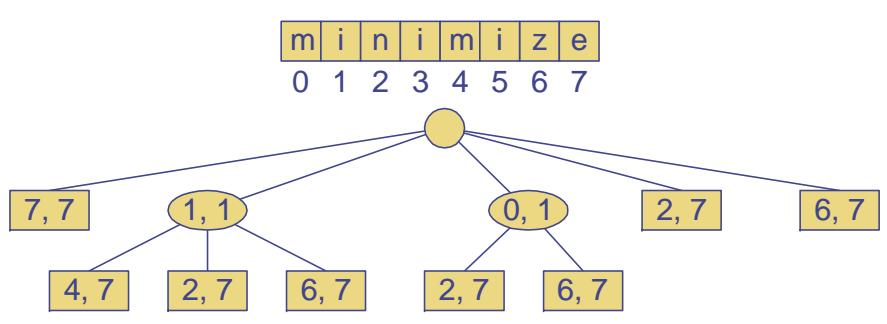
\includegraphics[width=0.9\linewidth]{images/suffix_trie_indexes}
		\caption{Suffix Trie with Index Representation}
		\label{fig:suffixtrieindexes}
	\end{minipage}
\end{figure}


\subsection{Laufzeitverhalten / Speicherplatz}
\begin{description}
	\item[n] totale Länge der Strings in S
	\item[m] Länge des Pattern
	\item[d] Grösse des Alphabets
\end{description}
\begin{table}[h]
	\centering
	\begin{tabu} to \linewidth {l l}
		\toprule
		Beschreibung & Big Oh \\
		\midrule
		Speicherverbrauch & $\mathcal{O}(n)$ \\
		Suchen, Einfügen, Löschen & $\mathcal{O}(dm)$ \\
		Erstellen des Trie & $\mathcal{O}(n)$ \\		\bottomrule
	\end{tabu}
	\caption{Big Oh Tries}
\end{table}

\subsection{Implementierung}
 \begin{lstlisting}
 public class TrieMultimap<V> implements Multimap<String, V> {

 	private TrieNode<V> root;

 	private enum Mutation {
 		INSERT, REMOVE
 	};

 	public TrieMultimap() {
 		this.root = new TrieNode<V>();
 	}

 	// Returns the first value for a given key. null if key is not found
 	public V find(String key) {
 		TrieNode<V> result = find(root, key);
 		if (result != null)
 		return result.getValues().get(0);
 		else
 		return null;
 	}

 	// return Iterator over all values. If key is not found: Iterator without next
 	public Iterator<V> findAll(String key) {
 		TrieNode<V> result = find(root, key);
 		if (result != null)
	 		return result.getValues().iterator();
 		else
	 		return new LinkedList<V>().iterator();
 	}

 	private TrieNode<V> find(TrieNode<V> node, String keySubstr) {
 		if (keySubstr.length() == 0) {
 			return node;
 		}
 		for (TrieNode<V> child : node.getChilds()) {
 			if (keySubstr.startsWith(child.getKeySubstr())) {
 				keySubstr = keySubstr.substring(child.getKeySubstr().length());
 				return find(child, keySubstr);
 			}
 		}
 		return null;
 	}

 	// Inserts a key/value pair into the multimap.
 	public void insert(String key, V value) {
 		TrieNode<V> result = find(root, key);
 		if (result != null) {
 			result.getValues().add(value);
 		} else {
	 		mutate(Mutation.INSERT, root, key, 0, value);
	 	}
	 }

	 private boolean mutate(Mutation operation, TrieNode<V> node, String key, int keyIndex, V value) {
	 	if (key.length() == keyIndex) {
	 		// found the node!
	 		if (operation == Mutation.INSERT) {
	 			node.getValues().add(value);
	 		} else { // REMOVE
		 		node.getValues().clear();
		 	}
		 	return true;
		}
		for (TrieNode<V> child : node.getChilds()) {
		 	if (child.getKeySubstr().charAt(0) == key.charAt(keyIndex)) {
		 		if (child.getKeySubstr().length() > 1) { // a compressed node?
		 			child = decompress(node, child);
		 		}
		 		boolean result = mutate(operation, child, key, ++keyIndex, value);
		 		compress(node, child);
		 		return result;
		 	}
		 }

		 // there is no corresponding child:
		 if (operation == Mutation.INSERT) {
		 	TrieNode<V> newNode = new TrieNode<>();
		 	newNode.setKeySubstr(key.substring(keyIndex, keyIndex + 1));
		 	node.getChilds().add(newNode);
		 	mutate(Mutation.INSERT, newNode, key, ++keyIndex, value);
		 	compress(node, newNode);
		 } else { // REMOVE
		 return false; // not found
		}
		return false;
	}

	private TrieNode<V> decompress(TrieNode<V> node, TrieNode<V> child) {
		// insert an additional, single-char node (de-compressing):
		TrieNode<V> newChild = new TrieNode<>();
		newChild.setKeySubstr(child.getKeySubstr().substring(0, 1));
		child.setKeySubstr(child.getKeySubstr().substring(1));
		newChild.getChilds().add(child);
		node.getChilds().add(newChild);
		node.getChilds().remove(child);
		return newChild;
	}

	private void compress(TrieNode<V> node, TrieNode<V> child) {
		if ((child != root) && (child.getChilds().size() == 1)
		&& (child.getValues().isEmpty())) {
			// compress:
			TrieNode<V> childOfChild = child.getChilds().get(0);
			child.setKeySubstr(child.getKeySubstr().concat(childOfChild.getKeySubstr()));
			child.getValues().addAll(childOfChild.getValues());
			child.getChilds().addAll(childOfChild.getChilds());
			child.getChilds().remove(childOfChild);
			return;
		}
		if (child.getChilds().isEmpty() && (child.getValues().isEmpty())) {
			// this is a removed node:
			node.getChilds().remove(child);
			return;
		}
	}

	// Removes all values for a given key.
	public void remove(String key) {
		TrieNode<V> result = find(root, key);
		if (result != null) {
			mutate(Mutation.REMOVE, root, key, 0, null);
		} else {
		return;
		}
	}

	public int size() {
		return size(root);
	}

	// return Number of values in this node and its child nodes.
	private int size(TrieNode<V> element) {
		int size = 0;
		for (TrieNode<V> child : element.getChilds()) {
			size += size(child);
		}
		size += element.getValues().size();
		return size;
	}
}
\end{lstlisting}

\section{Dynamische Programmierung}
Bei der dynamischen Programmierung geht es darum, auf die Lösungen von Subproblemen (die während dem Lösen entstehen) aufzubauen, um das ganze Problem zu lösen. Dynamische Programmierung kann dann erfolgreich eingesetzt werden, wenn das Optimierungsproblem aus vielen gleichartigen Teilproblemen besteht und eine optimale Lösung des Problems sich aus optimalen Lösungen der Teilprobleme zusammensetzt

\subsection{Rucksack Problem}
\begin{enumerate}
	\item Das Rucksackproblem (NP Vollständig), lässt sich nur so schnell lösen, weil wir ganze Zahlen haben
	\item Annahme: die Objekte sind genau einmal vorhanden. Der Rucksack bietet Platz für 8kg.
	\item Man geht spaltenweise \textbf{von links nach rechts} und prüft welcher maximale Wert für ein Gewicht möglich ist. Achtung: Es können auch mehrere Werte zusammengezählt werden. Das Gewicht auf der X-Achse darf aber nie überschritten werden.
	\begin{itemize}
		\item Bsp. Gewicht = 6
		\item 6 = 7/3 + 4/2 + 3/1 $\rightarrow$ maximal 14
	\end{itemize}
	\item In einem ersten Schritt werden die grösstmöglichen Werte in die Tabelle abgefüllt.
	\item Solange kein grösserer Wert gefunden wird, wird der \textbf{maximale Wert pro Spalte beibehalten}. In der nächsten Spalte wird aber wieder von vorne begonnen.
	\item Ist die komplette Tabelle ausgefüllt, steht der maximal mögliche Wert ganz unten rechts.
	\item Wenn da nächste Subproblem keine Verbesserung bringt, geht man wieder zurück zum Optimum des letzten Subproblems und übernimmt diesen Wert. Dabei geht man so vor, dass man in einer \textbf{Spalte von unten nach oben geht, bis sich der Wert ändert}. Dieser Wert wird ebenfalls in den Rucksack gelegt.
	\item Das nächste Subproblem wird wie folgt bestimmt:
	\begin{itemize}
		\item Ausgehend vom gerade hinzugefügten Objekt, wird das \textbf{hinzugefügt Gewicht vom Gewicht auf der X-Achse abgezogen}. Man geht in der Tabelle also um x Spalten nach links. \\
		(z.B Gewicht = 7 $\Rightarrow$ 8/4 konnte hinzugefügt werden $\rightarrow$ Weiter bei Gewicht = 3)
		\item Solange sich das Gewicht in einer Spalte nicht ändert, wird innerhalb der Spalte nach oben verschoben. (Der Wert/kg hat ja keine Verbesserung gebracht)
	\end{itemize}
\end{enumerate}

\newpage

\begin{figure}[h]
\centering
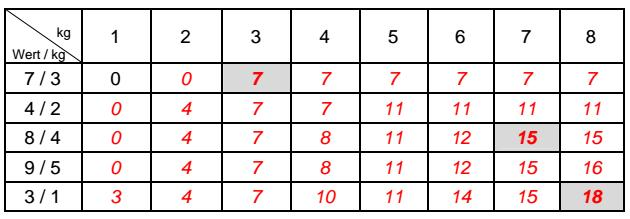
\includegraphics[width=0.8\linewidth]{images/dynamische_prog}
\caption{Dynamische Programmierung, Rucksackproblem}
\label{fig:dynamischeprog}
\end{figure}

\subsection{LCS: Longest Common Subsequence}
\begin{itemize}
	\item Finde die längste Subsequenz die in zwei Sequenzen enthalten ist, wobei die Subsequenz nicht an einem Stück sein muss (eher \textbf{Submenge}, kein Substring!). Die Reihenfolge der auftreten Zeichen muss aber der Reihenfolge im Text entsprechen.
	\item Der BruteForce Algorithmus läuft exponentiell mit $\mathcal{O}(2^n)$
	\item Beim Ansatz mit dynamischer Programmierung hat man eine Laufzeit von $\mathcal{O}(n \cdot m)$
	\item LCS mit dynamischer Programmierung wird z.B bei Versionsverwaltungstools verwendet
	\item Es gibt eine zusätzliche Reihe/Spalte mit dem Index -1, damit es möglich ist, KEINE Übereinstimmung abzubilden.
\end{itemize}

\clearpage

\subsection{Vorgehen}
\paragraph{Tabelle Aufbauen}
\begin{enumerate}
	\item $-1$ Zeile und Spalte Zeichen und Felder mit 0 initialisieren
	\item Tabelle aufbauen: Für alle Felder zeilenweise von \textbf{links nach rechts und oben nach unten}
	\begin{itemize}
		\item \textbf{Match}: Wenn die beiden Zeichen gleich sind: Zähle 1 zum Wert oben links (diagonal) hinzu
		\item \textbf{No Match}: Nimm ansonsten den maximalen Wert zwischen dem Wert links der aktuellen Position, oder oben von der aktuellen Position.
	\end{itemize}
\end{enumerate}

\paragraph{Lösungen finden} \hfill \\
Die LCS wird von  rechts nach links aufgebaut. Es kann verschiedene Lösungen geben, da man von nach jedem Match entweder der Reihe oder Kollonne folgen kann.
\begin{enumerate}
	\item Beginne unten rechts und prüfe ob die Zeichen gleich sind. 
	\item Wenn die Zeichen gleich sind, nimm das Zeichen in die LCS (von rechts nach links) und verschiebe diagonal nach \textbf{links/oben}.
	\item Wenn die Zeichen nicht gleich sind folge der \textbf{Kolonne oder Reihe}, bis die beiden Zeichen wieder gleich sind oder sich die Zahlen ändern.
	\item Wiederhole diese Schritte bis man ganz oben/links angekommen ist.
\end{enumerate}


\begin{figure}[h]
\centering
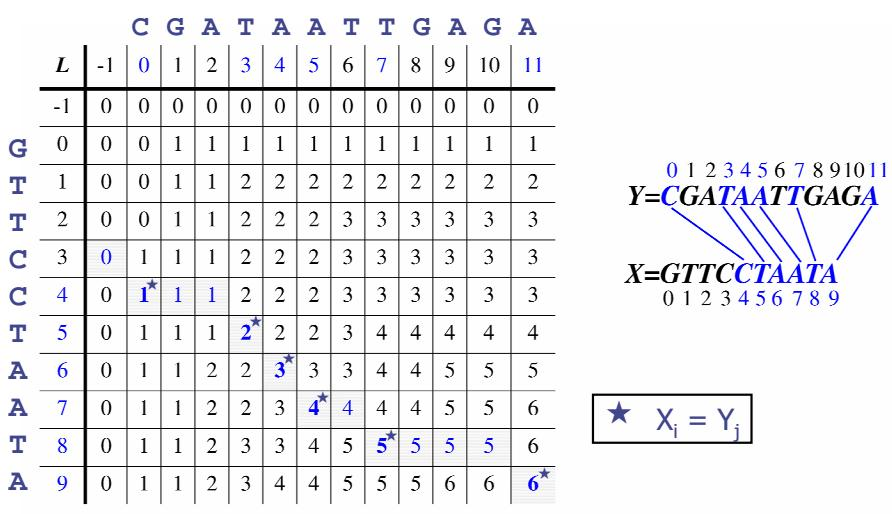
\includegraphics[width=\linewidth]{images/dynamische_prog_lcs}
\caption{Longest Common Subsequence}
\label{fig:dynamischeproglcs}
\end{figure}

\clearpage

\subsubsection{Implementierung}
\begin{lstlisting}
public class LCS {
	private int tableL[][]; // data array
	private String xStr;
	private String yStr;

	public int[][] calculateTable(final String xStr, final String yStr) {

		this.xStr = xStr;
		this.yStr = yStr;

		int n = xStr.length();
		int m = yStr.length();

		// +1 because of zero row/column
		tableL = new int[n + 1][m + 1];

		for (int i = 1; i <= n; i++) {
			for (int j = 1; j <= m; j++) {
				// - 1 because of the zero row/column
				if (xStr.charAt(i - 1) == yStr.charAt(j - 1)) {
					tableL[i][j] = tableL[i - 1][j - 1] + 1; 
				} else {
					tableL[i][j] = Math.max(tableL[i - 1][j], tableL[i][j-1]);
				}
			}
		}

		return tableL;
	}

	public List<String> findAll() {
		List<String> list = new LinkedList<>();
		Deque<Character> stack = new LinkedList<>();
		find(xStr.length(), yStr.length(), stack, list);
		List<String> result = new LinkedList<>();
		list.stream().sorted().distinct().forEach(str -> result.add(str));
		return result;
	}

	private void find(final int xPos, final int yPos, Deque<Character> stack, List<String> stringList) {
		if ((xPos == 0) || (yPos == 0)) { // reached the end?
			stringList.add(stack.toString());
			return;
		} else {
			if (xStr.charAt(xPos - 1) == yStr.charAt(yPos - 1)) {
				stack.push(xStr.charAt(xPos - 1));
				find(xPos - 1, yPos - 1, stack, stringList);
				stack.pop();
			}
			if (tableL[xPos - 1][yPos] == tableL[xPos][yPos]) {
				find(xPos - 1, yPos, stack, stringList);
			}
			if (tableL[xPos][yPos - 1] == tableL[xPos][yPos]) {
				find(xPos, yPos - 1, stack, stringList);
			}
		}
	}
}
\end{lstlisting}

\section{Graphen}
\subsection{Terminologie}
\begin{description}
	\item[G: Graph] Ein Paar (V,E). Besteht aus einem Set von Knoten und einer Collection von Kanten.
	\item[V: Vertizes] Ein Knoten
	\item[E: Edges] Eine Kante, enthält ein Paar von Vertizes
	\item[n] Anzahl Vertizes
	\item[m] Anzahl Kanten (\textbf{min}: $m=n-1$ (Liste), \textbf{max}: $m = \frac{n\cdot(n-1)}{2}$ (vollvermascht)). Mit $n-1$ Kanten lässt sich der ganze Graph verbinden (Ring)
	\item[gerichtete Kanten] Ein Knoten des Edges ist der Ursprung und der andere das Ziel. Die Kante wird als Pfeil dargestelt
	\item[ungerichtete Kanten] Ein ungeorneter Knoten Paar
	\item[gerichteter Graph] Alle vorhandenen Edges sind gerichet
	\item[ungerichteter Graph] Alle vorhandenen Edges sind ungerichtet
	\item[End-Vertizes] Endpunkt einer Kante. Eine Kante ist \lstinline|inzident| in einem Knoten (enden)
	\item[Adjazente] Benachbarte Knoten sind adjazent
	\item[Grad eines Vertex] Anzahl inzidenter Kanten. Wie viele Kanten mit einem anderen Knoten verbunden sind.
	\item[Parallele Kanten] Zwei Kanten zwischen zwei Knoten, die eine Schleife bilden \\
	\item[Schleife] Eine Kante mit dem gleichen Ursprung und Ziel \\
	\item[Connected] Ein Graph ist connected, falls zwischen allen Vertizes ein Pfad existiert.
\end{description}

\begin{figure}[h]
	\centering
	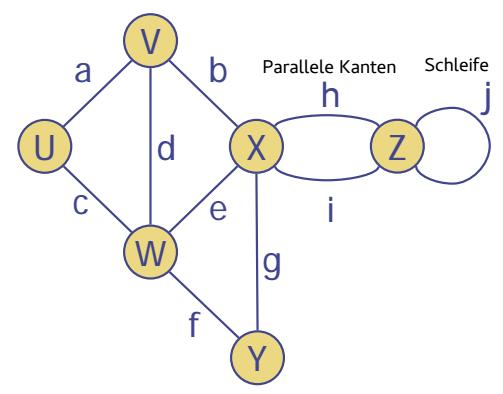
\includegraphics[width=0.4\linewidth]{images/terminologie}
	\caption{Parallele Kanten und Schleifen}
	\label{fig:terminologie}
\end{figure}

\subsubsection{Subgraphen}
\begin{description}
	\item[Subgraph] Alle Kanten und Vertizes des Subgraphen sind eine Teilmenge des Graphen
	\item[Aufspannender Subgraph] Ein aufspannender Subgraph enthält alle Vertizes des Graphen, jedoch nicht alle Kanten.
\end{description}

\subsubsection{Tree und Forest}
\begin{description}
	\item[Tree] Ist ein Graph der connected ist und keine Zyklen aufweist
	\item[Forest] Ist ein ungerichter Graph ohne Zyklen der aus Trees besteht.
	\item[Spanning Tree] Ist ein connected, nicht eindeutiger (Pfade können ändern), loopfreier Tree.
\end{description}

\subsubsection{Pfad und Zyklen}
\begin{description}
	\item[Pfad] Beginnt und Endet mit einem Vertex. (Einfacher Pfad = rot, Nicht einfacher Pfad = grün)
	\item[Zyklus] Ended mit einer Kante. Ein Zyklus verbindet implizit den letzten Vertex mit dem ersten. Ein einfacher Zyklus besucht nie zweimal den gleichen Vertex. (Einfacher Zyklus = rot, Nicht einfacher Zyklus = grün)
\end{description}
\begin{figure}[ht!]
	\centering
	\begin{minipage}[t]{0.4\textwidth}
		\centering
		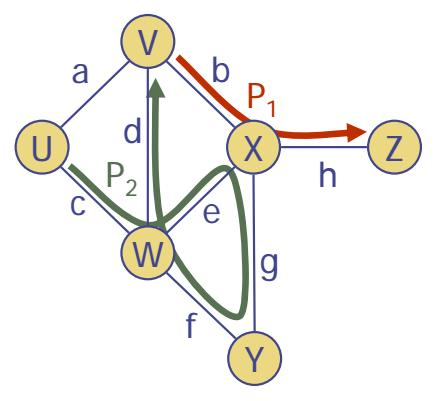
\includegraphics[width=0.9\linewidth]{images/graph_pfad}
		\caption{Pfad}
		\label{fig:graphpfad}
	\end{minipage}
	\begin{minipage}[t]{0.4\textwidth}
		\centering
		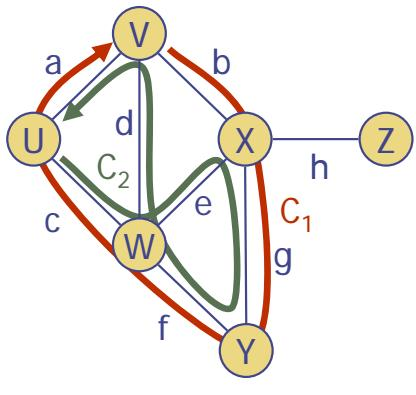
\includegraphics[width=0.9\linewidth]{images/graph_zyklus}
		\caption{Zyklus}
		\label{fig:graphzyklus}
	\end{minipage}
\end{figure}

\clearpage

\subsection{Kanten-Listen Struktur}
\begin{itemize}
	\item Grundsätzlich gibt es Objekte für die Vertices und die Edges
	\item Man hält sich je eine Sequenz für Vertices und eine für Edges
	\item Jedes Vertex Objekt hält eine Referenz auf die Position in der Vertex Sequenz
	\item Jedes Edge Objekt hält eine Referenz auf den Ursprungs- und Ziel Vertex, sowie eine Referenz auf seine Position in der Kanten-Struktur.
	\item Beim Einfügen kann der neue Vertex einfach am Ende der Liste angefügt werden. 
	\item Beim Löschen muss die gesamte Liste Liste von Kanten nach dem gesuchten Vertext durchsucht werden. 
	\item Die Kanten Listen Sturktur \textbf{wird selten verwendet}
\end{itemize}
\begin{figure}[h!]
\centering
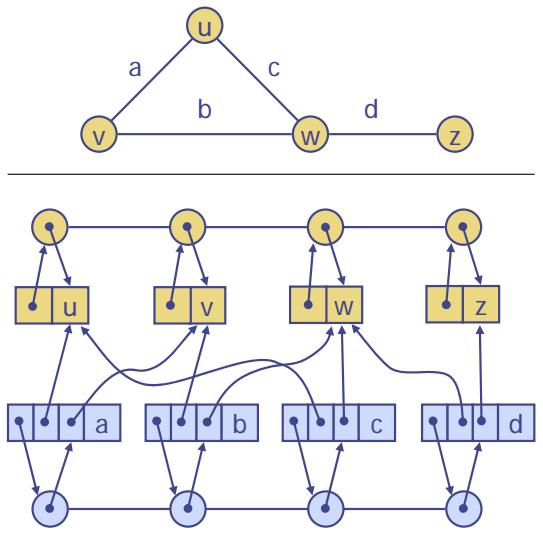
\includegraphics[width=0.5\linewidth]{images/graph_kanten_listen}
\caption{Kanten-Listen Struktur}
\label{fig:graphkantenlisten}
\end{figure}

\subsection{Adjazenz-Listen Struktur}
\begin{itemize}
	\item Baut auf der Kanten-Listen Struktur auf, mit der Erweiterung einer Inzidenz-Sequenz für jeden Vertex. Diese enthält die Positionen auf die erweiterten Kantenobjekte der inzidenten Kanten.
	\item Wird immer verwendet wenn man Mutation in dem Graphen macht
	\item Jedes Kanten Objekt hält eine Referenz auf den Ursprungs- und Ziel Vertex
	\item \textbf{Benötig sehr wenig Platz}, auch bei vielen Kanten/grossen Graphen.
\end{itemize}
\begin{figure}[h!]
\centering
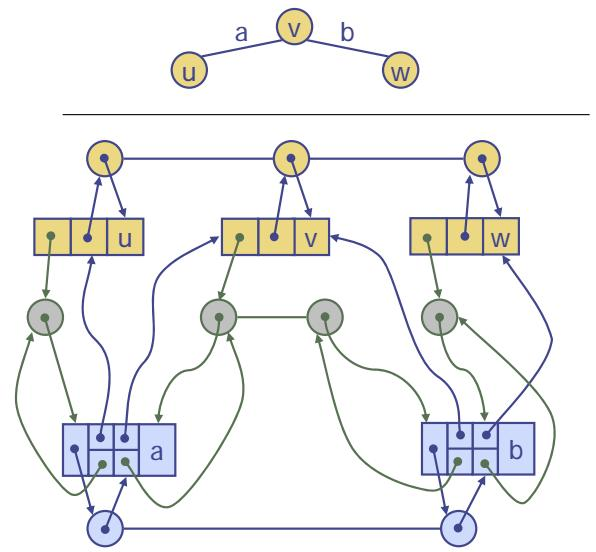
\includegraphics[width=0.5\linewidth]{images/graph_adjazenz_listen}
\caption{Adjazenz Listen Struktur}
\label{fig:graphadjazenzlisten}
\end{figure}

\subsection{Adjazenz-Matrix Struktur}
\begin{itemize}
	\item Baut auf der Kanten-Listen Struktur auf, mit der Erweiterung, dass die Vertex Objekte einen Index in die Adjazenz Matrix halten.
	\item Ist besonders für den lesenden Zugriff geeignet
	\item Kann \textbf{Anfragen zur Nachbarschaft sehr schnell} beantworten, benötigt jedoch mehr Platz
\end{itemize}
\begin{figure}[h!]
\centering
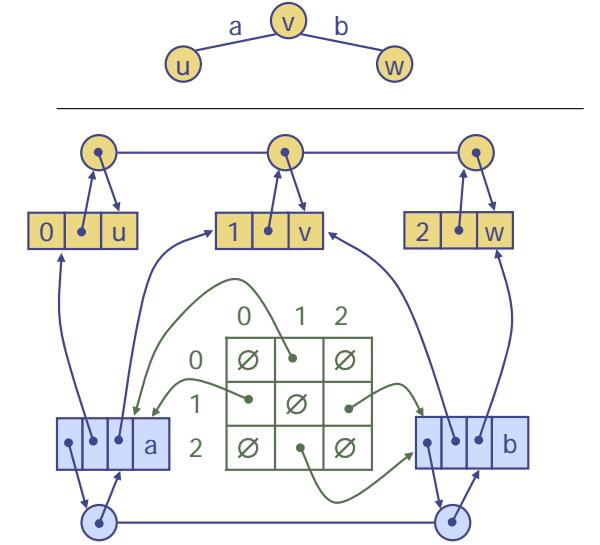
\includegraphics[width=0.5\linewidth]{images/graph_adjazenz_matrix}
\caption{Adjazenz-Matrix Struktur}
\label{fig:graphadjazenzmatrix}
\end{figure}

\subsection{Laufzeiten}
\begin{itemize}
	\item n Vertizes
	\item m Kanten
	\item keine parallelen Kanten
	\item keine Schleifen
\end{itemize}
\begin{table}[h]
	\centering
	\begin{tabu} to \linewidth {l l l l}
		\toprule
		Operation & Kanten Liste & Adjazenz Liste & Adjazenz Matrix\\
		\midrule
		Space & $\mathcal{O}(n+m)$ & $\mathcal{O}(n+m)$ & $\mathcal{O}(n^2)$   \\
		incidentEdges(v) & $\mathcal{O}(m)$ & $\mathcal{O}(dev(v))$ & $\mathcal{O}(n)$   \\
		areAdjacent(v, w) & $\mathcal{O}(m)$ & $\mathcal{O}(min(deg(v), deg(w))$ & $\mathcal{O}(1)$   \\
		insertVertex(o) & $\mathcal{O}(1)$ & $\mathcal{O}(1)$ & $\mathcal{O}(n^2)$   \\
		insertEdge(v, w, o) & $\mathcal{O}(1)$ & $\mathcal{O}(1)$ & $\mathcal{O}(1)$   \\
		removeVertex(v) & $\mathcal{O}(m)$ & $\mathcal{O}(deg(v))$ & $\mathcal{O}(n^2)$   \\
		removeEdge(e) & $\mathcal{O}(1)$ & $\mathcal{O}(1)$ & $\mathcal{O}(1)$   \\
		\bottomrule
	\end{tabu}
	\caption{Laufzeiten von Graph Operationen}
\end{table}

\subsection{Implementierung}
\begin{lstlisting}
// Graph
public class Graph<T extends Comparable<T>> extends Observable {
	
	private ArrayList<Node<T>> nodes;
	private Stack<Node<T>> stack;
	
	public Graph() {
		nodes = new ArrayList<Node<T>>();
		stack = new Stack<Node<T>>();
	}
	
	public Node<T> getNode(int indx) {
		return nodes.get(indx);
	}
	
	public void addNode(Node<T> n) {
		if (nodes.contains(n)) {
			return; // list is a set !
		}
		nodes.add(n);
	}
	
	// DFS
	public ArrayList<Node<T>> depthFirstSearch(Node<T> from, Node<T> to) {
		from.setMark(true);
		stack.push(from);
		if (from == to) {
			return new ArrayList<Node<T>>(stack);
		}
		for (Node<T> n : from.getConnectedNodes()) {
			System.out.println(from.getObject() + ": " + n.getObject() + " ");
			if (!n.isMarked()) {
				ArrayList<Node<T>> path = depthFirstSearch(n, to);
				if (path != null) {
					return path;
				}
			}
		}
		stack.pop();
		return null;
	}
	
	// BFS
	public ArrayList<Node<T>> breadthFirstSearch(Node<T> from, Node<T> to) {
		ArrayList<IntermediatePath<T>> queue = new ArrayList<>();
		IntermediatePath<T> ip = new IntermediatePath<>(null, from);
		queue.add(ip);
		from.setMark(true);
		while (queue.size() > 0) {
			ip = queue.remove(0);
			if (ip.current == to) {
				ArrayList<Node<T>> path = new ArrayList<>();
				do {
					path.add(0, ip.current);
				} while ((ip = ip.previous) != null);
				return path;
			}
			for (Node<T> it : ip.current.getConnectedNodes()) {
				if (!it.isMarked()) {
					it.setMark(true);
					IntermediatePath<T> newIP = new IntermediatePath<T>(ip, it);
					queue.add(newIP);
					System.out.print("  previous: " + newIP.previous.current.getObject()
					+ "  current: " + newIP.current.getObject());
				}
			}
		}
		return null;
	}
}
\end{lstlisting}


\begin{lstlisting}
// Node
public class Node<T extends Comparable<T>> {
	
	// Connected neighbour nodes
	private ArrayList<Node<T>> linked;
	private T obj;
	
	public Node(T obj) {
		this.obj = obj;
		linked = new ArrayList<Node<T>>();
	}
	
	public ArrayList<Node<T>> getConnectedNodes() {
		return linked;
	}
	
	public void connectTo(Node<T> n) {
		ListIterator<Node<T>> it = linked.listIterator();
		while(it.hasNext()) {
			Node<T> listNode = it.next();
			int compareResult = n.getObject().compareTo(listNode.getObject());
			if (compareResult == 0) {
				return; // list is a set!
			} else if (compareResult < 0) {
				it.previous();
				it.add(n);
				return;
			}
		}
		// Node has not yet been inserted
		linked.add(n);
	}
	
}
\end{lstlisting}


\newpage

\section{DFS und BFS}
\subsection{DFS: Depth First Search}
\begin{itemize}
	\item Tiefensuche
	\item Mit dem DFS Algorithmus werden durch Graphen traversiert
	\item Die mit \lstinline|DISCOVERY| markierten und besuchten Kanten bilden einen Spanning Tree
	\item Der DFS kann verwendet werden um einen \textbf{Pfad und Zyklung zu finden}. Ebenfalls kann eine Topologische Sortierung damit erstellt werden.
	\item In einem gerichteten Graph, geht der DFS Algorithmus so tief wie möglich und macht anschliessend ein Backtracking. 
	\begin{enumerate}
		\item Setzt in einem ersten Schritt alle Edges und Vertizes auf \lstinline|UNEXPLORED|
		\item Führt rekursiv für alle Vertizes den DFS Algorithmus durch
		\item Die Incident Kanten sind aufsteigend sortiert!
		\item Wenn die Kante nicht bereits besucht wurde, geht man zum gegenüberliegenden Knoten und setzt ihn auf \lstinline|DISCOVERY|.
		\item Geht man von einem Knoten aus zurück, fängt man den nächsten Iterationsschritt, bei dem Knoten an, der besucht wurde, bevor man zurück ging.
		\item Terminiert der rekursive DFS Algorithmus wird noch einmal jeder Vertex überprüft, ob er \lstinline|UNEXPLORED| ist. Gibt es immer noch \lstinline|UNEXPLORED| Edges, kann der Graph nicht connected sein, da der Algorithmus garantiert alle verbundenen Knoten besucht.
		\item Gibt es eine Kante mit dem \lstinline|BACK| Label, hat man einen Zyklus
	\end{enumerate}
\end{itemize}

\begin{figure}[h!]
	\centering
	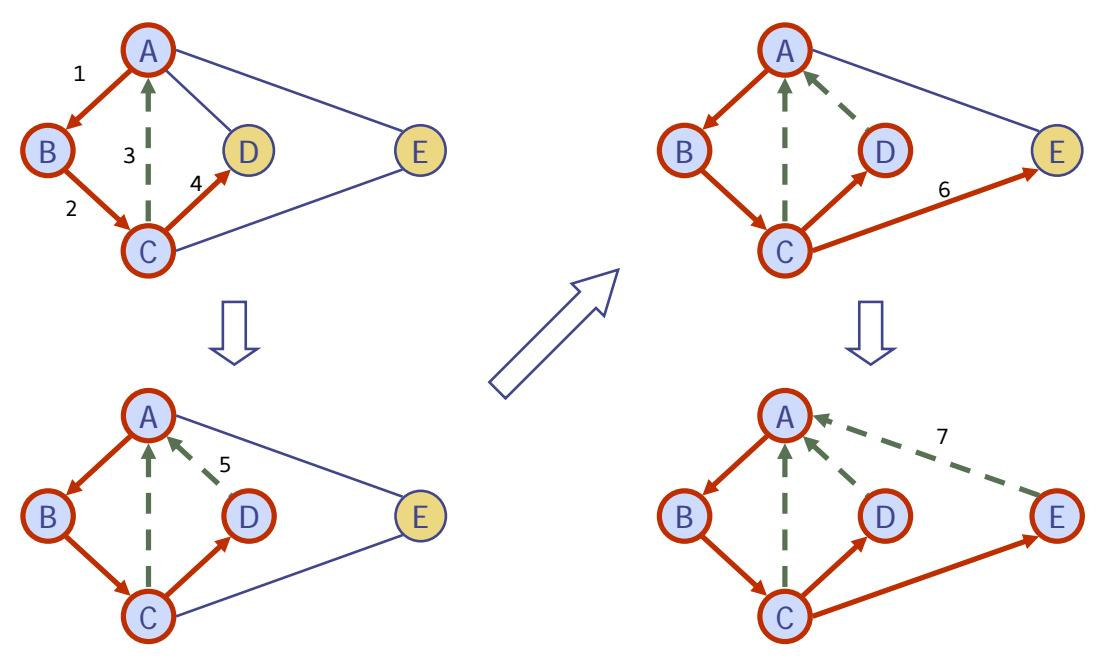
\includegraphics[width=0.7\linewidth]{images/dfs_example}
	\caption{Depth First Search}
	\label{fig:dfsexample}
\end{figure}

\begin{figure}[h!]
	\centering
	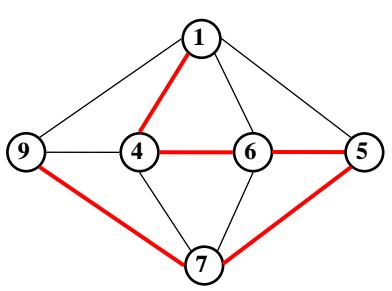
\includegraphics[width=0.5\linewidth]{images/tiefensuche}
	\caption{Tiefensuche}
	\label{fig:tiefensuche}
\end{figure}


\begin{algorithm}[h!]
	\KwData{Graph G}
	\KwResult{Labeling of the edges of G as discovery edges and back edges}
	\ForAll{u in G.vertices()}
	{
		$setLabel(u, UNEXPLORED)$
	}
	\ForAll{e in G.edges()}
	{
		$setLabel(e, UNEXPLORED)$		
	}
	\ForAll{v in G.vertices()}{
		\If{$getLabel(v) == UNEXPLORED$}{
			$DFS(G,v)$
		}
		\Else {
			\tcp{not conencted}
		}
	}
	\caption{DFS(G)}
\end{algorithm}

\begin{algorithm}[h!]
	\KwData{Graph G and a Start vertex v of G}
	\KwResult{Labeling of the edes of G in the connected component of v as discovery edges and back edges}
	$setLabel(v, VISITED)$ \\
	\ForAll{e in G.incidentEdges(v)}
	{
		\If{$getLabel(e) == UNEXPLORED$} {
			$w \leftarrow opposite(v,e)$ \\
			\If{$getLabel(w) == UNEXPLORED$} {
				$setLabel(e, DISCOVERY)$ \\
				$DFS(G,W)$
			}
			\Else {
				$setLabel(e, BACK)$
			}
		}
	}
	\caption{DFS(G,v)}
\end{algorithm}



\clearpage

\subsection{BFS: Breadth First Search}
\begin{itemize}
	\item Breitensuche
	\item Der BFS Algorithmus findet im Gegensatz zum DFS den \textbf{direktestens Pfad} zu einem Knoten. Dies ist meist auch der kürzeste. Dies muss aber nicht gezwungermassen sein, da z.B mehrere kleine Pfade schneller sind wie der direkte. (Beispiel SBB)
	\item Der BFS Algorithmus besucht jeden Vertex genau ein mal.
	\item Der BFS Algorithmus initialisiert die Knoten und Edges auf die selbe Weise wie der DFS. 
	\item Der BFS Algorithmus ist im Gegensatz zum DFS \textbf{nicht rekursiv}.
\end{itemize}
\begin{figure}[h]
\centering
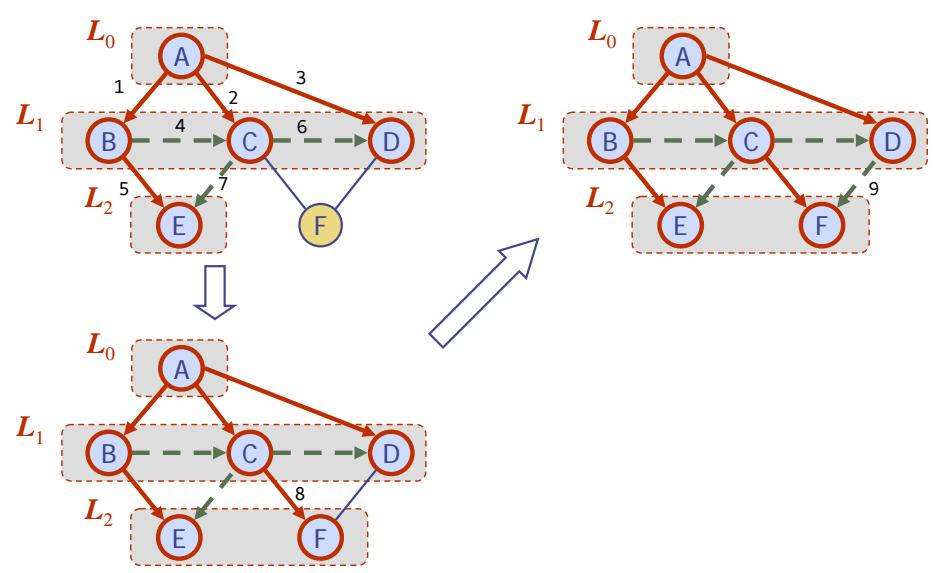
\includegraphics[width=0.7\linewidth]{images/bfs_example1}
\caption{Breath First Search}
\label{fig:bfsexample1}
\end{figure}

\begin{figure}[h!]
	\centering
	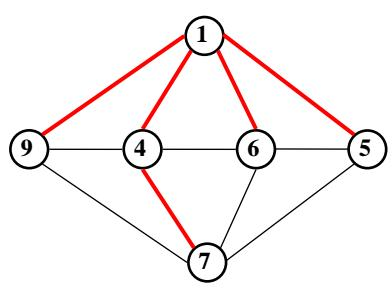
\includegraphics[width=0.5\linewidth]{images/breath_first}
	\caption{Breitensuche}
	\label{fig:breathfirst}
\end{figure}


\begin{algorithm}[H]
	$L_0 \leftarrow new empty sequence$ \\
	$L_0.insertLast(s)$ \\
	$setLabel(s, VISITED)$ \\
	$i \leftarrow 0$ \\
	\While{$\lnot L_i.isEmpty$} {
		\ForAll{v in $L_i$.elements()}
		{
			\ForAll{e in G.incidentEdges(v)}
			{
				\If{$getLabel(e) == UNEXPLORED$} {
					$w \leftarrow opposite(v,e)$ \\
					\If{$getLabel(w) == UNEXPLORED$} {
						$setLabel(e, DISCOVERY)$ \\
						$setLabel(w, VISITED)$ \\
						$L_{i+1}.insertLast(w)$ \\
					}
					\Else {
						$setLabel(e, BACK)$
					}
				}
			}
		}
	}

	\caption{BFS(G,s)}
\end{algorithm}



\subsection{DFS vs. BFS}
\begin{itemize}
	\item n Vertizes
	\item m Kanten
	\item keine paralleleln Kanten
	\item keine Schleifen
\end{itemize}
\begin{table}[h]
	\centering
	\begin{tabu} to \linewidth {X c c}
		\toprule
		Beschreibung & Depth First Search & Breadth First Search \\
		\midrule
		Laufzeit & $\mathcal{O}(n+m)$ & $\mathcal{O}(n+m)$   \\
		Aufspannender Wald, Verbundene Komponenten, Pfade, Zyklen & $\checkmark$ & $\checkmark$  \\
		Kürzester Pfad &  & $\checkmark$   \\
		Biconnected Komponenten & $\checkmark$ &   \\
		\bottomrule
	\end{tabu}
	\caption{Laufzeiten von Graph Operationen}
\end{table}

\section{Gerichtete Graphen}
Ein gerichteter Graph (Digraph, Directed Graph) ist ein Graph, dessen Kanten alle gerichtet sind. Das bedeuted, dass die Kanten nur \textbf{unidirektional} begehbar sind. Die In und Out Katen werden in separaten Adjazenz Listen geführt.  


\subsection{Laufzeiten}
Wenn die In und Out Kanten in separaten Adjazenz Listen geführt werden, verläuft die Laufzeit proportional zur Grösse der Liste.

\begin{table}[h]
	\centering
	\begin{tabu} to \linewidth {l c}
		\toprule
		Beschreibung & Laufzeiten \\
		\midrule
		Strong Connectivity Algorithmus & $\mathcal{O}(n+m)$ \\
		Transitiver Abschluss & $\mathcal{O}(n(n+m))$ \\
		Floyd-Warshalls Algorihtmus & $\mathcal{O}(n^3)$ \\
		Topologische Sortierung & $\mathcal{O}(n+m)$ \\
		Topologische Sortiereung mit DFS & $\mathcal{O}(n+m)$ \\
		\bottomrule
	\end{tabu}
	\caption{Laufzeiten von Graph Operationen}
\end{table}


\subsection{Strong Connectivity}
Bei gerichteten Graphen ist es nicht garantiert, dass alle Vertizes erreichbar sind. Bei einem Graphen der streng verbunden, kann jedoch \textbf{jeder Vertex alle anderen Vertizes erreichen}. Mit dem Strong Connectivy Algoritmus kann mit nur \textbf{zwei Tiefensuchen} herausgefunden werden, ob ein Graph streng verbunden ist. 
\begin{enumerate}
	\item Wähle einen Vertex v in G und führe eine Tiefensuche durch. Wenn es einen nicht besuchten Vertex gibt, gib \lstinline|false| zurück
	\item Erstelle eine Kopie von G mit umgekehrten Kanten
	\item Wähle den gleichen Vertex v in G' und führe eine Tiefensuche durch. Wenn es einen nicht besuchten Vertex gibt, gib \lstinline|false| zurück. Ansonsten \lstinline|true|.
\end{enumerate}

\clearpage

\subsection{DFS und BFS}
Sowohl die Tiefensuche als auch die Breitensuche kann für gerichtete Graphen angepasst werden.
\begin{description}
	\item[discovery] Baumkanten/Discovery sind Kanten des Pfades
	\item[back] Rückkanten sind Verbindungen zu einem Vorgänger des selben Astes (der bereits auf DISCOVERY gesetzt ist) \\
	(ACHTUNG gäbe es eine Verbindung von 2 nach 8, wäre es keine back-Kante sondern eine Cross Kante $\rightarrow$ Anderer Ast)
	\item[forward] Vorwärtskanten sind Verbindungen zu einem Nachfolger im Baum (der bereits auf DISCOVERY gesetzt ist)
	\item[cross] Kreuzkanten sind alle übrigen Kanten (z.B andere Pfad)
\end{description}

\begin{figure}[h]
\centering
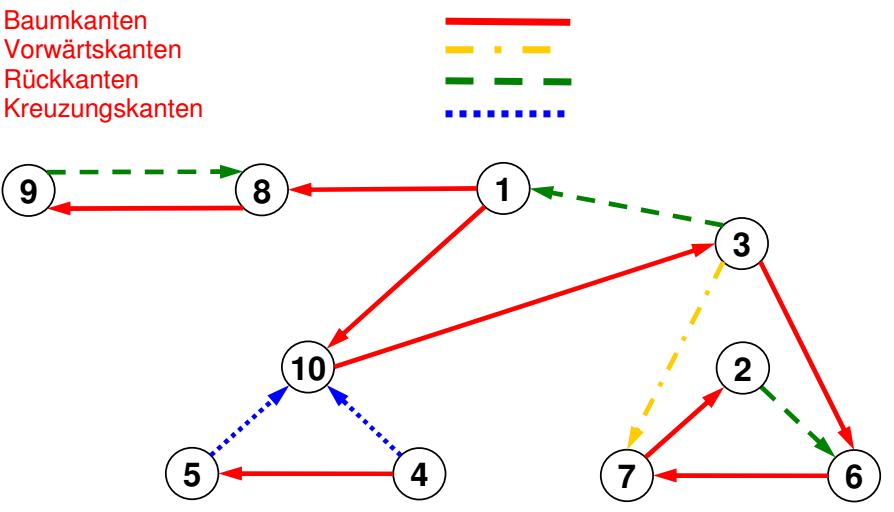
\includegraphics[width=\linewidth]{images/digraph_dfs}
\caption{Digraph DFS}
\label{fig:digraphdfs}
\end{figure}

\clearpage

\subsection{Transitiver Abschluss}
Der Transitive Abschluss erweitert einen bestehenden Graphen um \textbf{''Abkürzungen''}, sofern sowieso ein Pfad von einem Vertex zum anderen Vertex besteht. Wenn dies der Fall ist, bietet der Transitive Abschluss den direkten Weg zwischen zwei Vertex. 

\begin{figure}[h]
	\centering
	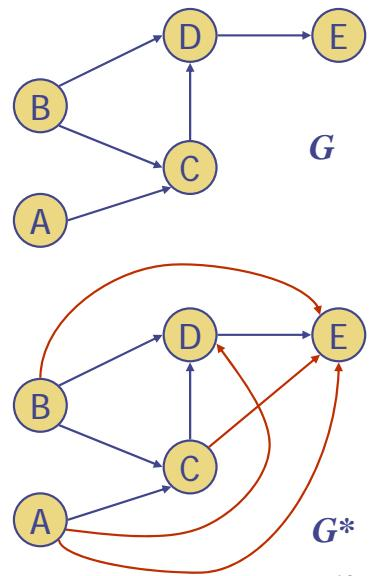
\includegraphics[width=0.3\linewidth]{images/transitive_abschluss}
	\caption{Transitive Abschluss}
	\label{fig:transitiveabschluss}
\end{figure}

\clearpage

\subsection{Floyd-Warshalls Algorithmus}
Der Floyd Warshalls Algorithmus erstellt einen Transitiven Abschluss für einen Graphen G. Er basiert auf dynamischer Programmierung. Das bedeutet, dass man auf die Lösung des vorangegangenen Problems aufsetzt. (z.B Nutzen des roten Pfeils, siehe Abbildung \ref{fig:floyd-warshal}) In einem transitiven Abschluss sind alle Knoten direkt mit einander verbunden, welche so oder so über andere Knoten erreicht hätten werden können.

\subsubsection{Vorgehen}
\begin{enumerate}
	\item Nummeriere alle Vertices der Reihe nach ($v_1$ bis $v_i$)
	\item Ausgehend vom ersten Vertex $v_i$ 
	\begin{enumerate}
		\item Folge allen ausgehenden Edges zum nächsten Vertex und merke diesen.
		\item Folge allen eingehenden Edges und verbinde diese Vertices jeweils $\rightarrow$ mit den Vertices im vorherigen Schritt, sofern diese nicht bereits verbunden sind.
	\end{enumerate}
	\item Sind alle Vertices in diesem Schritt verbunden, geht man zum nächsten Vertex $v{i+1}$ und wiederholt die Prozedur. 
	\item Die neu gezeichneten Edges \textbf{bleiben für die folgenden Schritte bestehenden} und müssen ebenfalls beachtet werden (Dynamische Programmierung)
\end{enumerate}

\begin{figure}[ht!]
	\centering
	\begin{minipage}[t]{0.4\textwidth}
		\centering
		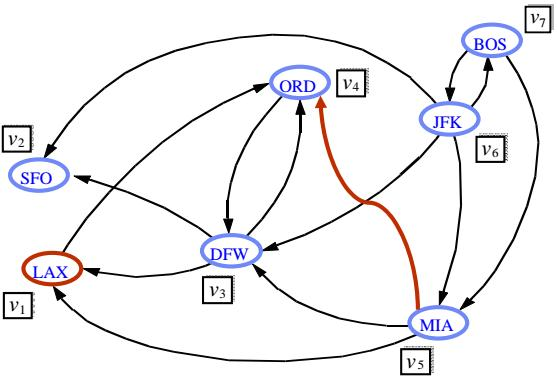
\includegraphics[width=\linewidth]{images/floyd-warshal}
		\caption{Schritt 1}
		\label{fig:floyd-warshal}
	\end{minipage}
	\begin{minipage}[t]{0.4\textwidth}
		\centering
		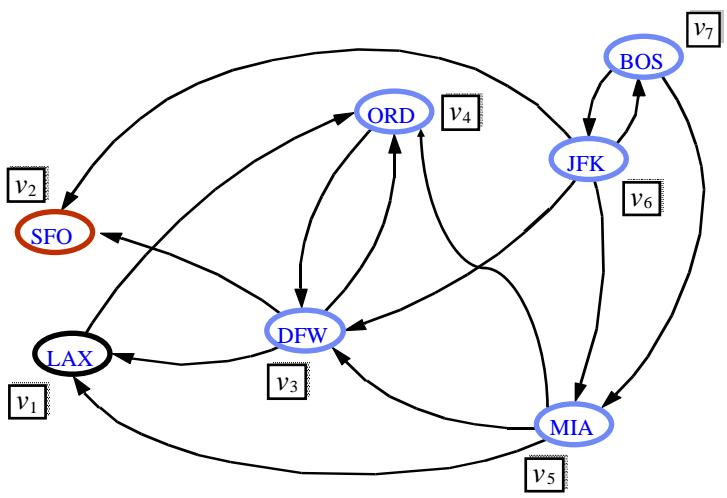
\includegraphics[width=\linewidth]{images/floyd-warshal_v2}
		\caption{Schritt 2}
		\label{fig:floyd-warshalv2}
	\end{minipage}
	\begin{minipage}[t]{0.4\textwidth}
		\centering
		\includegraphics[width=\linewidth]{images/floyd-warshal_v3}
		\caption{Schritt 3}
		\label{fig:floyd-warshalv3}
		\end{minipage}
\end{figure}

\begin{algorithm}[H]
	\KwData{digraph G}
	\KwResult{transitive closure G* of G}
	$i \leftarrow 1$ \\
	\ForAll{v in $G$.vertices()}
	{
		denote $v$ as $v_i$ \\
		$i \leftarrow i + 1$
	}
	$G_0 \leftarrow G$ \\
	\For{$k \leftarrow 1$ \KwTo $n$} 
	{
		$G_k \leftarrow G_{k-1}$ \\
		\For{$i \leftarrow 1$ \KwTo $n(i\neq k)$} 
		{
			\For{$j \leftarrow 1$ \KwTo $n(j\neq i, k)$} 
			{
				\If{$G_{k-1}.areAdjacent(v_i, v_k) \land G_{k-1}.areAdjacent(v_k, v_j)$} 
				{
					\If{$\lnot G_k.areAdjacent(v_i, v_j)$} 
					{
						$G_k.insertDirectedEdge(v_i, v_j, k)$
					}
				}
			}
		}
	}	
	\Return $G_n$
	\caption{FloydWarshall(G)}
\end{algorithm}

\clearpage


\subsection{DAG: Directed Acyclic Graph}
Ein DAG \textbf{enthält keine gerichteten Zyklen}.

\subsection{Topolgische Sortierung}
Man spricht von einer Topologischen Ordnung, wenn die Vertizes so \textbf{nummeriert} werden, dass die gerichteten Kanten immer auf grössere Vertizes zeigen. Eine topologische Ordnung kann nur in DAG's (keine Zyklen) erstellt werden.  
\begin{itemize}
	\item Eine Topologische Sortierung wird zum Beispiel beim kompilieren von C++ Objekt Files benötigt. So kann garantiert werden, dass keine unaufgelöste Referenzen existieren.
	\item Gleiches gilt bei Package Manager mit Dependencies.
	\item Der Algorithmus für die Topologische Sortierung läuft mit $\mathcal{O}(n+m)$
\end{itemize}

\begin{algorithm}[H]
	$H \leftarrow G$ \\
	$n \leftarrow G.numVertices()$ \\
	\While{$H is not empty$}
	{
		Let $v$ be a vertex with no outgoing edges \\
		Label $v \leftarrow n$ \\
		$n \leftarrow n -1  $ \\
		Remove $v$ from $H$
	}
	\caption{TopologicalSort(G)}
\end{algorithm}

\newpage

\subsubsection{Vorgehen}
Gibt es Zyklen, gibt es keine Topologische Sortierung und es ist kein DAG.
\begin{itemize}
	\item Nimm den ersten Vertex, gemäss der Sortierung von \lstinline|G.vertices()|.
	\item Mache eine Tiefensuche:
	\begin{enumerate}
		\item Besuche die Vertices (gemäss gegebener Sortierung von \lstinline|v.outgoingEdges()|), solange es einen gerichteten Edge hat und der Zielvertex noch nicht besucht wurde. 
		\item Wenn es nicht mehr weitergeht, mache ein Backtracking, bis es einen neuen Weg gibt. 
		\item Beim Backtracking werden die Nummern gesetzt. Angefangen beim Maximum (Anzahl Vertices)
	\end{enumerate}
\end{itemize}

\begin{figure}[ht!]
	\centering
	\begin{minipage}[t]{0.4\textwidth}
		\centering
		\includegraphics[width=\linewidth]{images/dag_topological_sort}
		\caption{Schritt 1}
		\label{fig:dagtopologicalsort}
	\end{minipage}
	\begin{minipage}[t]{0.4\textwidth}
		\centering
		\includegraphics[width=\linewidth]{images/dag_topological_sort_2}
		\caption{Nach dem ersten Backtracking}
		\label{fig:dagtopologicalsort2}
	\end{minipage}
	\begin{minipage}[t]{0.4\textwidth}
			\centering
		\includegraphics[width=\linewidth]{images/dag_topological_sort_3}
		\caption{Nach dem zweiten Backtracking}
		\label{fig:dagtopologicalsort3}
	\end{minipage}
	\begin{minipage}[t]{0.4\textwidth}
		\centering
		\includegraphics[width=\linewidth]{images/dag_topological_sort_4}
		\caption{Topologische Sortierung}
		\label{fig:dagtopologicalsort4}
\end{minipage}
\end{figure}



\subsubsection{DAG Implementierung}
Topologische Tiefensuche. \hfill \\
\begin{algorithm}[H]
	\KwData{DAG G}
	\KwResult{topological ordering of G}
	$n \leftarrow G.numVertices()$ \\
	\ForAll{u in $G$.vertices()}
	{
		$setLabel(u, UNEXPLORED)$
	}
	\ForAll{e in $G$.edges()}
	{
		$setLabel(e, UNEXPLORED)$
	}
	\ForAll{v in $G$.vertices()}
	{
		\If{$getLabel(v) = UNEXPLORED$}
		{
			$topologicalDFS(G, v)$
		}
	}
	\caption{topologicalDFS(G)}
\end{algorithm}

\begin{algorithm}[H]
	\KwData{graph G and a start vertex v of G}
	\KwResult{labeling of the vertices of G in the connected component of v}
	$setLabel(v, VISITED)$ \\
	\ForAll{e in $G.outgoingEdges(v)$}
	{
		\If{$getLabel(e) = UNEXPLORED$}
		{
			$w \leftarrow opposite(v,e)$ \\
			\If{$getLabel(w) = UNEXPLORED$} 
			{	
				$setLabel(e, DISCOVERY)$ \\
				$topologicalDFS(G, w)$
			}
			\Else
			{
				$e$ is a forward or cross edge
			}
		}
	}
	Label $v$ with topological number $n$ \\
	$n \leftarrow n - 1$
	\caption{topologicalDFS(G,v)}
\end{algorithm}

\clearpage

\begin{lstlisting}[caption=Directed DFS in Java]
	public void directedDFS() {
		vertices.forEach(v -> vertexLabeling.put(v, VertexState.UNEXPLORED));
		edges.forEach(e -> edgeLabeling.put(e, EdgeState.UNEXPLORED));
		
		vertices.forEach(v -> {
			if (vertexLabeling.get(v) == VertexState.UNEXPLORED) {
				directedDFS(v);
			}
		});
	}
	
	public void directedDFS(Vertex vertex) {
		vertexLabeling.put(vertex, VertexState.VISITED);
		
		outgoingEdges(vertex).forEach(e -> {
			
			if (edgeLabeling.get(e) == EdgeState.UNEXPLORED) {		
				Vertex opposite = opposite(vertex, e);
				if (vertexLabeling.get(opposite) == VertexState.UNEXPLORED) {
					edgeLabeling.put(e, EdgeState.DISCOVERY);
					displayOnGVS();
					directedDFS(opposite);
				} else {
					setKindOfEdge(vertex, e);
					displayOnGVS();
				}
			}
		});
	}
	
	private void setKindOfEdge(Vertex startVertex, Edge e) {
		Vertex endVertex = opposite(startVertex, e);
		if (path.contains(endVertex)) {
			// BACK
		} else if (subtreeNodes.get(startVertex).contains(endVertex)) {
			// FORWARD
		} else {
			// CROSS
		}
	}
\end{lstlisting}


\section{Shortest Path Trees}
\begin{itemize}
	\item Der SPT Algorithmus benötigt einen gewichteten Graphen
	\item In einem gewichteten Graphen hat jede Kante einen assoziierten numerischen Wert, das sogenannte Gewicht
	\item Typische Anwendungsfälle sind Routing, Verkehr oder Navigation im Auto
	\item Ein kürzester Pfad hat zwei Eigenschaften
	\begin{enumerate}
		\item Ein Teilweg eines kürzesten Weges ist selbst auch ein kürzester Weg
		\item Es existiert ein Baum von kürzesten Wegen von einem Start Vertex zu allen anderen Vertizes
	\end{enumerate}
\end{itemize}

\subsection{Laufzeiten}
\begin{table}[h]
	\centering
	\begin{tabu} to \linewidth {l c}
		\toprule
		Beschreibung & Laufzeiten \\
		\midrule
		Dijkstra Algorithmus mit Adjazenz Listen Struktur & $\mathcal{O}((n+m) \cdot log(n))$\\
		Bellman Ford & $\mathcal{O}(n\cdot m)$ \\
		DAG basierter Ansatz & $\mathcal{O}(n+m)$\\
		\bottomrule
	\end{tabu}
	\caption{Laufzeiten von Graph Operationen}
\end{table}

\clearpage

\subsection{Dijkstra Algorithmus}
Der Dijkstra Algorithmus berechnet die Distanzen zu allen Vertizes von einem Start Vertex aus. Dazu müssen \textbf{drei Annahmen} getroffen werden:
\begin{enumerate}
	\item Der Graph ist verbunden
	\item Die Kanten sind ungerichtet
	\item Die Kantengewichte sind \textbf{nicht negativ}
\end{enumerate}
Der Dijkstra Algorithmus ist ein Greedy Algorithmus, der immer den Vertex mit der kleinsten Distanz der Cloud hinzufügt. Um trotzdem mit negativen Gewichten umgehen zu können, könnte man die Gewichte einfach um das grösste negative Gewicht shiften. Dabei muss aber beachtet werden, dass man die Wertebereiche der Datentypen nicht überschreitet.

\begin{description}
	\item[Relaxation(Entspannung)] Wenn ein besserer Pfad gefunden wurde, werden die umliegenden Vertizes aktualisiert.
\end{description}

\subsubsection{Vorgehen}
\begin{enumerate}
	\item Die Standard Gewichte der Knoten ist $\infty$. Ausnahme ist der Start Vertex, dieser hat das Gewicht von 0.
	\item Aktualisiere alle Gewichte der umliegenden Knoten, falls es nun einen kürzeren Pfad zu einem Knoten gibt. (Immer \textbf{aufaddieren}: Knoten Gewicht + Kanten Gewicht)
	\item Der Wolke wir jener Vertex hinzugefügt, welcher noch nicht in der Wolke ist und den kleinsten Wert aufweist. Er muss aber von der Wolke erreichbar sein.
	\item Fahre fort mit dem Knoten der in die Wolke hinzugefügt wurde
	\item Wiederhole diese Schritte, bis alle Vertex in der Wolke sind. 
	\item Der Shortest Path ist nun der rote Pfad
\end{enumerate}

\vfill

\begin{figure}[h]
\centering
\includegraphics[width=0.6\linewidth]{images/dijkstra_algorithm}
\caption{Dijkstra Algorithmus}
\label{fig:dijkstraalgorithm}
\end{figure}

\subsubsection{Implementierung}
Der Dijkstra Algorithmus verwendet eine adaptierbare Priority Queue, wobei der Key die Distanz und das Value der Vertex ist. Die Eigenschaft der APQ ist es, dass man die Keys verändern kann. (Im Gegensatz zur Priority Queue)

\begin{lstlisting}[caption=Dijkstra Algorithmus]
public void distances(AdjacencyListGraph<V, E> graph, Vertex<V> s) {
	AdaptablePriorityQueue<Integer, Vertex<V>> apq = 
			new HeapAdaptablePriorityQueueGVS<Integer, Vertex<V>>();
	Map<Vertex<V>, Integer> distances = new LinkedHashMapGVS<Vertex<V>, Integer>();
	Map<Vertex<V>, Entry<Integer, Vertex<V>>> locators =
			new LinkedHashMap<Vertex<V>, Entry<Integer, Vertex<V>>>();
	Map<Vertex<V>, Edge<E>> parents = new LinkedHashMapGVS<Vertex<V>, Edge<E>>();
	gvs.set(apq, distances, parents);
	
	for (Vertex<V> v : graph.vertices()) {
		if (v == s) {
			distances.put(v, 0);
			// root node has no parents
			parents.put(v, null);
		} else {
			// set default distance to infinity
			distances.put(v, Integer.MAX_VALUE);
		}
		// add distance and vertex
		Entry<Integer, Vertex<V>> entry = apq.insert(distances.get(v), v);
		locators.put(v, entry);
	}

	while (!apq.isEmpty()) {
		// take next vertex out of the queue (removeMin) -> Kehrwert =  cloud
		AdjacencyListGraph<V, E>.MyVertex<V> cloudVertex = 
				(AdjacencyListGraph<V, E>.MyVertex<V>) (apq.removeMin().getValue());
				
		for (Edge<E> incidentEdge : cloudVertex.incidentEdges()) {
			Vertex<V> oppositVertex = graph.opposite(cloudVertex, incidentEdge);
			// calculate new weight: last vertex + edge weight
			int newWeight = distances.get(cloudVertex) + (Integer) incidentEdge.get(WEIGHT);
			if (newWeight < distances.get(oppositVertex)) {
				// relaxion
				distances.put(oppositVertex, newWeight);
				parents.put(oppositVertex, incidentEdge);
				apq.replaceKey(locators.get(oppositVertex), newWeight);
			}
		}
	}
}
\end{lstlisting}

\clearpage

\subsection{Bellman-Ford}
\begin{itemize}
	\item Im Gegensatz zum Dijkstra Algorithmus, funktioniert der BF Algorithmus \textbf{auch mit negativen Gewichten}
	\item Es gibt zwei voraussetzungen
	\begin{itemize}
		\item gerichtete Kanten
		\item keine negativ-gewichtete Schlaufen!
	\end{itemize}
	\item Die Laufzeit ist jedoch deutlich schlechter: $\mathcal{O}(n\cdot m)$
	\item Der BF Algorithmus \textbf{iteriert über alle Kanten} des Graphen und nicht nur um die umliegenden Kanten.
\end{itemize}

\begin{figure}[h]
\centering
\includegraphics[width=0.9\linewidth]{images/bellman-ford}
\caption{Bellman-Ford Algorithmus}
\label{fig:bellman-ford}
\end{figure}


\subsubsection{Implementierung}
\begin{algorithm}[H]
	\ForAll{v in $G.vertices()$}
	{
		\If{$v = s$}
		{
			
			$setDistance(v,0)$ 
		}
		\Else {
			$setDistance(v,\infty)$ 
		}
		\For{$i \leftarrow 1$ \KwTo $n -1 $} {
			$u \leftarrow G.origin(e)$ \\	
			$z \leftarrow G.opposite(u, e)$ \\
			$r \leftarrow getDistance(u) + weight(e)$ \\
			\If{$r < getDistance(z)$}
			{
				$setDistance(z,r)$
			}
		} 
	}
\caption{BellmanFord(G,s)}
\end{algorithm}

\subsection{DAG basierter Algorithmus}
\begin{itemize}
	\item Funktioniert wie der BF Algorithmus mit negativ-gewichteten Kanten
	\item Ein DAG ist ein gerichteter Graph \textbf{ohne Zyklen}
	\item Benutzt eine topologische Reihenfolge
	\item Ist sehr schnell: $\mathcal{O}(n+m)$
\end{itemize}

\begin{figure}[h]
\centering
\includegraphics[width=0.7\linewidth]{images/dag_shortest_path}
\caption{DAG Shortest Path}
\label{fig:dagshortestpath}
\end{figure}


\section{Minimum Spanning Tree}
\begin{itemize}
	\item Anwendungsfälle sind Kommunikationsnetzwerke und Transportnetzwerke
	\item Ein minimaler Spanning Tree ist ein Subset von Kanten in einem ungerichteten, bidirektionalen, gewichteten Graphen der alle Knoten ohne Zyklen und mit den kleinsten Kosten verbindet.
\end{itemize}

\begin{description}
	\item[Schlaufen Eigenschaft] \hfill \\
	Gibt es eine Kante $e$ die noch nicht zum MST gehört und ein tieferes Gewicht hat, wie mindestens eine Kante im MST, ersetzt sie die Kanten mit dem höheren Gewicht, sofern sie den MST zu einer Schleife formt.
	\item[Aufteilungseigenschaft] Die Kante mit dem \textbf{kleinsten Gewicht} muss Teil des Pfades sein
\end{description}

\subsection{Kruskal Algorithmus}
\begin{itemize}
	\item Der Kruskal Algorithmus merkt sich einen Forest von Trees. 
	\item Eine Kante ist akzeptiert, wenn sie zwei Trees verbindet. 
	\item Eine Priority Queue speichert die Kanten ausserhalb der Wolke (Key: Gewicht, Value: Kante).
\end{itemize}
\begin{figure}[ht!]
	\centering
	\begin{minipage}[t]{0.4\textwidth}
		\centering
		\includegraphics[width=0.9\linewidth]{images/kruskal_s1}
		\caption{Step 1}
		\label{fig:kruskals1}
	\end{minipage}
	\begin{minipage}[t]{0.4\textwidth}
		\centering
		\includegraphics[width=0.9\linewidth]{images/kruskal_s2}
		\caption{Step 2}
		\label{fig:kruskals2}
	\end{minipage}
\end{figure}

\begin{figure}[ht!]
	\centering
	\begin{minipage}[t]{0.4\textwidth}
		\centering
		\includegraphics[width=0.9\linewidth]{images/kruskal_s3}
		\caption{Step 3}
		\label{fig:kruskals3}
	\end{minipage}
	\begin{minipage}[t]{0.4\textwidth}
		\centering
		\includegraphics[width=0.9\linewidth]{images/kruskal_s4}
		\caption{Step 4}
		\label{fig:kruskals4}
	\end{minipage}
\end{figure}

\subsection{Prim-Jarnik's Algorithmus}
Ist ein modifizierter Dijkstra Algorithmus. Wir nehmen einen beliebigen Vertex s und generieren den minimalen Spanning Tree als Wolke von Vertizes von s. Danach speichern wir zu jedem Vertex ein label d(v) = kleinste Gewichtung einer Kante, welche v mit einem Vertex der Wolke verbindet. Bei jedem Schritt werden folgende Dinge durchgeführt:

\subsubsection{Vorgehen}
\begin{enumerate}
	\item Die Standard Gewichte der Knoten ist $\infty$. Ausnahme ist der Start Vertex, dieser hat das Gewicht von 0.
	\item Aktualisiere alle Gewichte der umliegenden Knoten mit den \textbf{Gewichten der Kante}. Hier wird nichts aufaddiert.
	\item Der Wolke wir jener Vertex hinzugefügt, welcher noch nicht in der Wolke ist und den kleinsten Wert aufweist. Er muss aber von der Wolke erreichbar sein.
	\item Fahre fort mit dem Knoten der in die Wolke hinzugefügt wurde
	\item Wiederhole diese Schritte, bis alle Vertex in der Wolke sind. 
	\item Der Minimal Spanning Tree ist nun der rote Pfad
\end{enumerate}

\begin{figure}[h!]
	\centering
	\includegraphics[width=0.9\linewidth]{images/prim-jarnik-algo}
	\caption{Prim-Jarnik's Algorithmus}
	\label{fig:prim-jarnik-algo}
\end{figure}

\clearpage

\subsection{Borůvka's Algorithmus}
Der Borůvka's Algorithmus arbeitet wie der Kruskal Algorithmus, mit einem Unterschied: Hier gibt es \textbf{für jede Cloud eine Priority Queue}. Dieser Algorithmus wird selten verwendet und ist \textbf{nur historisch relevant}.

\subsection{Laufzeit}
\begin{table}[h]
	\centering
	\begin{tabu} to \linewidth {l c}
		\toprule
		Beschreibung & Laufzeiten \\
		\midrule
		Partition-based Kruskal & $\mathcal{O}(m \cdot log(n))$\\
		Prim-Jarnik's & $\mathcal{O}(m \cdot log(n))$\\
		Borůvka's & $\mathcal{O}(m \cdot log(n))$\\
		\bottomrule
	\end{tabu}
	\caption{Laufzeiten von Graph Operationen}
\end{table}



\appendix

% Code Listings
\lstlistoflistings

% List of figures
\listoffigures

% List of tables
\listoftables

% Bibliography
\bibliographystyle{plain} 
\bibliography{literatur}

\end{document}
